\documentclass[a4paper,fleqn,12pt]{article}
\usepackage[utf8]{inputenc}
\usepackage[brazilian]{babel}

\usepackage[T1]{fontenc}
%\usepackage[utf8]{inputenc}
\usepackage[brazilian]{babel}
\usepackage[left=2.5cm,right=2.5cm,top=3cm,bottom=2.5cm]{geometry}
\usepackage{mathtools}
%\usepackage{amsthm}
\usepackage{amsmath}
\usepackage{nccmath}
\usepackage{amssymb}
\usepackage{amsfonts}
\usepackage{physics}
\usepackage{dsfont}
%\usepackage{mathrsfs}

\usepackage{titling}
\usepackage{indentfirst}

\usepackage{bm}
\usepackage[dvipsnames]{xcolor}
\usepackage{cancel}

\usepackage{xurl}
\usepackage[colorlinks=true]{hyperref}

\usepackage{float}
\usepackage{graphicx}
\usepackage{tikz}
\usepackage{caption}
\usepackage{subcaption}

%%%%%%%%%%%%%%%%%%%%%%%%%%%%%%%%%%%%%%%%%%%%%%%%%%%

\newcommand{\eps}{\epsilon}
\newcommand{\vphi}{\varphi}
\newcommand{\cte}{\text{cte}}

\newcommand{\N}{\mathbb{N}}
\newcommand{\Z}{\mathbb{Z}}
\newcommand{\Q}{\mathbb{Q}}
\newcommand{\R}{\mathbb{R}}
\newcommand{\C}{\mathbb{C}}
\renewcommand{\H}{\hat{H}}
\newcommand{\intR}{\int_{-\infty}^{\infty}}

\newcommand{\0}{\vb{0}}
\newcommand{\1}{\mathds{1}}
\newcommand{\E}{\vb{E}}
\newcommand{\B}{\vb{B}}
\renewcommand{\v}{\vb{v}}
\renewcommand{\r}{\vb{r}}
\renewcommand{\k}{\vb{k}}
\newcommand{\p}{\vb{p}}
\newcommand{\q}{\vb{q}}
\newcommand{\F}{\vb{F}}

\renewcommand{\a}{\hat{a}}
\renewcommand{\b}{\hat{b}}
\renewcommand{\c}{\hat{c}}
\newcommand{\nn}{\hat{n}}

\newcommand{\gf}[2]{\ev{\ev{#1 : #2}}}
\newcommand{\zub}[2]{\ev{\comm{#1}{#2}_\mp}}

\newcommand{\s}[1]{\mathcal{#1}}
%\newcommand{\prodint}[2]{\left\langle #1 , #2 \right\rangle}
\newcommand{\cc}[1]{\overline{#1}}
\newcommand{\Eval}[3]{\eval{\left( #1 \right)}_{#2}^{#3}}

\newcommand{\unit}[1]{\; \mathrm{#1}}

\newcommand{\n}{\medskip}
\newcommand{\e}{\quad \mathrm{e} \quad}
\newcommand{\ou}{\quad \mathrm{ou} \quad}
\newcommand{\virg}{\, , \;}
\newcommand{\ptodo}{\forall \,}
\renewcommand{\implies}{\; \Rightarrow \;}
%\newcommand{\eqname}[1]{\tag*{#1}} % Tag equation with name

\setlength{\droptitle}{-8em}


\title{\Huge{\textbf{Assignments 8, 9 e 11}}}
\author{Mateus Marques}

\begin{document}

\maketitle

\section{Assigment 8}

\subsection{Problem 1}

Temos que $\{ \a_i, \a_j^\dagger \} = \delta_{ij}$, $\{\a_i, \a_j^\dagger \a_j \} = \delta_{ij} a_j$ e $\{ \a_i^\dagger, \a_j^\dagger \a_j \} = - \delta_{ij} \a^\dagger_j$. Além disso, das relações $[\a, \b \c] = \{\a, \b\} \c - \b \{\a, \c\}$ ou $[\a \b, \c] = \a \{\b, \c\} - \{\a, \c\} \b$, temos que
$$
[\a_1, \a_1^\dagger \a_2] = \{\a_1, \a_1^\dagger\} \a_2 - \a_1^\dagger \{\a_1, \a_2\} = \a_2 - 0 = \a_2.
$$

\subsubsection{}

Com a hamiltoniana $\H = \sum_{k=1}^2 \eps_k \a^\dagger_k \a_k - \lambda(\a_1^\dagger \a_2 + \a_2^\dagger \a_1)$, segue então que $[\a_1, \H] = \eps_1 \a_1 - \lambda \a_2$. Analogamente para $[\a_2, \H]$, obtemos da equação de Heisenberg:
\begin{ceqn} \label{eq:heisenberg1}
\begin{align}
i \dv{t}
\begin{pmatrix}
\a_1 \\ \a_2
\end{pmatrix}
=
\begin{pmatrix}
\eps_1 & -\lambda \\
-\lambda & \eps_2
\end{pmatrix}
\begin{pmatrix}
\a_1 \\ \a_2
\end{pmatrix}
=
M
\begin{pmatrix}
\a_1 \\ \a_2
\end{pmatrix}.
\end{align}
\end{ceqn}
Por $M$ ser simétrica, sabemos que pode ser diagonalizada ortonormalmente. Assim, escrevemos $M = U \, \text{diag}(\omega_1, \omega_2) \, U^T$, onde parametrizamos
$$
U =
\begin{pmatrix}
\cos\theta & \sin\theta \\
-\sin\theta & \cos\theta
\end{pmatrix}.
$$

\subsubsection{} \label{sec:sol-nonint}

A solução da equação \ref{eq:heisenberg1} é dada por $\vb{\a}(t) = U \, \text{diag}(e^{-i\omega_1 t}, e^{-i\omega_2 t}) \, U^T \, \vb{\a}(0)$. Portanto
$$
\begin{pmatrix}
\a_1(t) \\ \a_2(t)
\end{pmatrix} =
\begin{pmatrix}
\cos \theta & \sin \theta \\
-\sin\theta & \cos\theta
\end{pmatrix}
\begin{pmatrix}
e^{-i\omega_1 t} \cos\theta & -e^{-i\omega_1 t}\sin\theta \\
e^{-i\omega_2 t} \sin\theta & e^{-i\omega_2 t}\cos\theta
\end{pmatrix}
\begin{pmatrix}
\a_1(0) \\ \a_2(0)
\end{pmatrix} =
$$
$$
\begin{pmatrix}
e^{-i\omega_1 t} \cos^2\theta + e^{-i\omega_2 t}\sin^2\theta & (e^{-i\omega_2 t} - e^{-i\omega_1 t}) \sin\theta \cos\theta \\
(e^{-i\omega_2 t} - e^{-i\omega_1 t}) \sin\theta \cos\theta & e^{-i\omega_2 t} \cos^2\theta + e^{-i\omega_1 t}\sin^2\theta
\end{pmatrix}
\begin{pmatrix}
\a_1(0) \\ \a_2(0)
\end{pmatrix}.
$$

\subsubsection{}

No limite em que $\lambda = 0$, a matriz $M$ já é diagonal. Nesse caso, temos que $U = \1$ e $\theta = 0$. Nesse caso, a solução se reduz a $\a_k(t) = e^{-i\eps_k t} \a_k(0)$, que é a solução da \textit{free-hamiltonian}, onde só existe uma oscilação de fase trivial.

\subsubsection{}

Com a solução obtida em \ref{sec:sol-nonint}, podemos calcular $\nn_k(t) = \a^\dagger_k(t) \a_k(t)$. Para o caso do $\nn_1$ temos
$$
\nn_1(t) =
\qty{ \qty[e^{i\omega_1 t} \cos^2\theta + e^{i\omega_2 t}\sin^2\theta ] \a_1^\dagger(0) + \qty[ (e^{i\omega_2 t} - e^{i\omega_1 t}) \sin\theta \cos\theta ] \a_2^\dagger(0) }
$$
$$
\times \, \qty{ \qty[e^{-i\omega_1 t} \cos^2\theta + e^{-i\omega_2 t}\sin^2\theta ] \a_1(0) + \qty[ (e^{-i\omega_2 t} - e^{-i\omega_1 t}) \sin\theta \cos\theta ] \a_2(0) }.
$$
Fazendo essa bagunça:
$$
\boxed{\nn_1(t)} =
\qty{\cos^4\theta + 2 \cos^2\theta \sin^2\theta \, \cos[(\omega_2 - \omega_1)t] + \sin^4\theta} \, \a^\dagger_1(0) \a_1(0) \; +
$$
$$
\qty{ 2 \sin^2\theta \cos^2\theta \, (1 - \cos[(\omega_2 - \omega_1) t]) } \, \a^\dagger_2(0) \a_2(0) \; +
$$
$$
\qty{ \sin\theta \cos\theta \qty[ \qty(1 + e^{i(\omega_2-\omega_1)t}) \sin^2\theta - \qty(1 - e^{-i(\omega_2-\omega_1)t} ) \cos^2\theta ] } \,
\a^\dagger_1(0) \a_2(0) \; +
$$
$$
\qty{ \sin\theta \cos\theta \qty[ \qty(1 + e^{-i(\omega_2-\omega_1)t}) \sin^2\theta - \qty(1 - e^{i(\omega_2-\omega_1)t} ) \cos^2\theta ] } \,
\a^\dagger_2(0) \a_1(0).
$$

\n

A expressão para $\nn_2(t)$ é obtida trocando $1 \leftrightarrow 2$.

%Agora podemos utilizar o fato que $\{\a_1, \a_2\} = 0$. Assim, as duas últimas linhas acima nos dão
%$$
%- \frac{i}{2} \sin(4\theta)  \sin[(\omega_2 - \omega_1) t ] \, \a^\dagger_1(0) \a_2(0).
%$$
%
%Portanto:
%$$
%\boxed{ \nn_1(t) } =
%\Big\{ \cos^4\theta + 2 \cos^2\theta \sin^2\theta \, \cos[(\omega_2 - \omega_1)t] + \sin^4\theta \Big\} \, \a^\dagger_1(0) \a_1(0) \; +
%$$
%$$
%\Big\{ 2 \sin^2\theta \cos^2\theta \, (1 - \cos[(\omega_2 - \omega_1) t]) \Big\} \, \a^\dagger_2(0) \a_2(0)
%\; - \; \qty{ \frac{i}{2} \sin(4\theta)  \sin[(\omega_2 - \omega_1) t ] } \, \a^\dagger_1(0) \a_2(0).
%$$

\subsection{Problem 2}

\subsubsection{}

Chamando $\lambda = V_d - V_x$, temos
$$
[\a_1, \H] = \eps \a_1 + \lambda (\a_1 \a^\dagger_1\a^\dagger_2 \a_2 \a_1  - \a^\dagger_1 \a_1 \a^\dagger_2 \a_2 \cancelto{0}{\a_1^2}) =
(\eps_1 + \lambda \a_2^\dagger \a_2) \, \a_1.
$$
Analogamente, $[\a_2, \H] = (\eps_2 + \lambda \a_1^\dagger \a_1) \, \a_2$.

\subsubsection{}

As equações de movimento são
\begin{ceqn}
\begin{align} \label{eq:eom-int}
\begin{cases}
\; i \dv{\a_1}{t} = (\eps_1 + \lambda \nn_2) \, \a_1 \\
\; i \dv{\a_2}{t} = (\eps_2 + \lambda \nn_1) \, \a_2,
\end{cases}
\end{align}
\end{ceqn}
onde $\nn_k = \a^\dagger_k \a_k$.

\subsubsection{}

Note que a equação de movimento para $\a_1^\dagger$ é
$$
i \dv{\a^\dagger_1}{t} = - (\eps_1 + \lambda \nn_2) \, \a^\dagger_1
$$
Perceba então que
$$
i \dv{\nn_1}{t} = i \dv{\a^\dagger_1}{t} \, \a_1 + \a^\dagger_1 \, i \dv{\a_1}{t} =
- (\eps_1 + \lambda \nn_2) \a^\dagger_1 \a_1 + \a^\dagger_1 (\eps_1 + \lambda \nn_2) \a_1
= 0.
$$
O mesmo vale para $\nn_2$. Portanto, $\nn_k(t) = \a_k^\dagger(0) \a_k(0)$ é um operador constante.

Com essa observação, \textit{à princípio}, é possível resolver as equações de movimento para $\a_1(t)$ e $\a_2(t)$ analiticamente. A solução é dada pela exponencial de um operador constante:
$$
\a_1(t) = e^{-i\qty[\eps_1 + \lambda \a_2^\dagger(0) \a_2(0)]} \a_1(0) \e
\a_2(t) = e^{-i\qty[\eps_2 + \lambda \a_1^\dagger(0) \a_1(0)]} \a_2(0).
$$

Agora, $\ev{\nn_k}(t) = \ev{\a^\dagger_k(0) \a_k(0)} = \cte$.

\subsubsection{}

Na aproximação de \textit{mean-field}, separamos $\H = \H_0 + \hat{V}$, onde $\H_0 = \sum_{k=1}^2 \eps_k \a^\dagger_k \a_k$ e $\hat{V} = \lambda \, \nn_1 \nn_2$. Então expandimos $\hat{V}$, substituindo $\nn_k = \ev{\nn_k} + \hat{\delta}_k$ e ignoraremos termos de segunda ordem $O(\hat{\delta}_k \hat{\delta_\ell})$.

O potencial de \textit{mean-field} é
$$
V_{\text{MF}} = \lambda \, \Big(\ev{\nn_1} \nn_2 + \ev{\nn_2} \nn_1 - \ev{\nn_1}\ev{\nn_2}\Big).
$$

Agora podemos calcular os comutadores $[\a_k, \H]$ e obter novamente as equações de movimento. Porém, outra maneira mais direta é fazer diretamente na equação exata \ref{eq:eom-int} a aproximação de \textit{mean-field} $n_k \a_\ell = \ev{n_k} \a_\ell$.

A solução é muito parecida com o que já obtivemos:
$$
\a_1(t) = e^{-i\qty[\eps_1 + \lambda \ev{\a_2^\dagger(0) \a_2(0)}]} \a_1(0) \e
\a_2(t) = e^{-i\qty[\eps_2 + \lambda \ev{\a_1^\dagger(0) \a_1(0)}]} \a_2(0).
$$


\section{Assignment 9}

\subsection{Problem 1}

Ah, é muito fácil substituir $G^R$ e $G^A$ nas equações e verificar que
$$
\qty[\dv{t} - H] G(\r t, \r' t') = \delta(\r-\r') \delta(t-t').
$$
Agora, temos que $G^R$ e $G^A$ são independentes pois $G^R(\r t, \r' t') = 0$ para $t < t'$ enquanto que $G^A(\r t, \r' t') = 0$ para $t > t'$.

\subsection{Problem 2}

Temos que
$$
\frac{1}{\omega + i \eta} = \frac{\omega}{\omega^2 + \eta^2} - i \pi \, \frac{\eta/\pi}{\omega^2 + \eta^2}.
$$
Integrando sobre uma função teste $f$, temos que
$$
\lim_{\eta \to 0} \intR \frac{f(\omega) \dd{\omega}}{\omega + i\eta} =
\lim_{\eta \to 0} \intR \frac{f(\omega) \, \omega \dd{\omega}}{\omega^2 + \eta^2} \; - \;
i \pi \, \lim_{\eta \to 0} \intR f(\omega) \, \frac{\eta/\pi}{\omega^2 + \eta^2} \dd{\omega}
$$
$$
= P.V. \intR \frac{f(\omega)}{\omega} \dd{\omega} - i \pi f(0).
$$
Isso mostra que
$$
\lim_{\eta \to 0} \, \frac{1}{\omega + i\eta} = P.V. \qty(\frac{1}{\omega}) - i \pi \delta(\omega).
$$


\section{Assignment 11}

\subsection{Problem 1}

Assumindo que $\Sigma^{(0)}(\omega^+) = \Lambda - i \Delta$, com $\Lambda$ e $\Delta$ constantes, temos que
$$
\cc{G}_{d\sigma}^R(\omega^+) =
\frac{\Big[\omega - \big(\eps_0 + \Lambda + U \ev{\nn_{d\cc{\sigma}}}\big) \Big] - i \Big[ \Delta + \eta \Big]}{\Big[\omega - \big(\eps_0 + \Lambda + U \ev{\nn_{d\cc{\sigma}}}\big) \Big]^2 + \Big[ \Delta + \eta \Big]^2}.
$$
Portanto
$$
\ev{\nn_{d\sigma}} = \int_{-\infty}^{\eps_F} A_{d\sigma}(\omega) \dd{\omega} = \frac{1}{\pi} \, \lim_{\eta \to 0} \int_{-\infty}^{\eps_F}
\frac{(\Delta + \eta) \, \dd{\omega}}{\Big[\omega - \big(\eps_0 + \Lambda + U \ev{\nn_{d\cc{\sigma}}}\big) \Big]^2 + \Big[ \Delta + \eta \Big]^2}
$$
$$
= \frac{1}{\pi} \, \int_{-\infty}^{\eps_F} \frac{1}{1 + \qty[\frac{\omega - (\cc{\eps}_0 + U \ev{\nn_{d\cc{\sigma}}})}{\Delta}]^2} \, \frac{\dd{\omega}}{\Delta}.
$$
Substituindo $\xi = \frac{\omega - (\cc{\eps_0} + U \ev{\nn_{d\cc{\sigma}}})}{\Delta}$ e aproximando a energia de Fermi $\eps_F \approx 0$, obtemos
$$
\ev{\nn_{d\sigma}} = \frac{1}{\pi} \, \int_{-\infty}^{-\frac{\cc{\eps}_0 + U \ev{\nn_{d\cc{\sigma}}}}{\Delta}} \frac{\dd{\xi}}{1 + \xi^2} =
\frac{1}{2} - \frac{1}{\pi} \, \arctan(\frac{\cc{\eps}_0 + U \ev{\nn_{d\cc{\sigma}}}}{\Delta}).
$$

\subsection{Problem 2}

Não entendi o comentário de tomar a média da iteração anterior no código do modelo de Anderson. Tempo 43:22 no vídeo da Aula 11.

\n\n\n\n

\begin{figure}[H]
\centering
\begin{subfigure}{.5\textwidth}
  \centering
  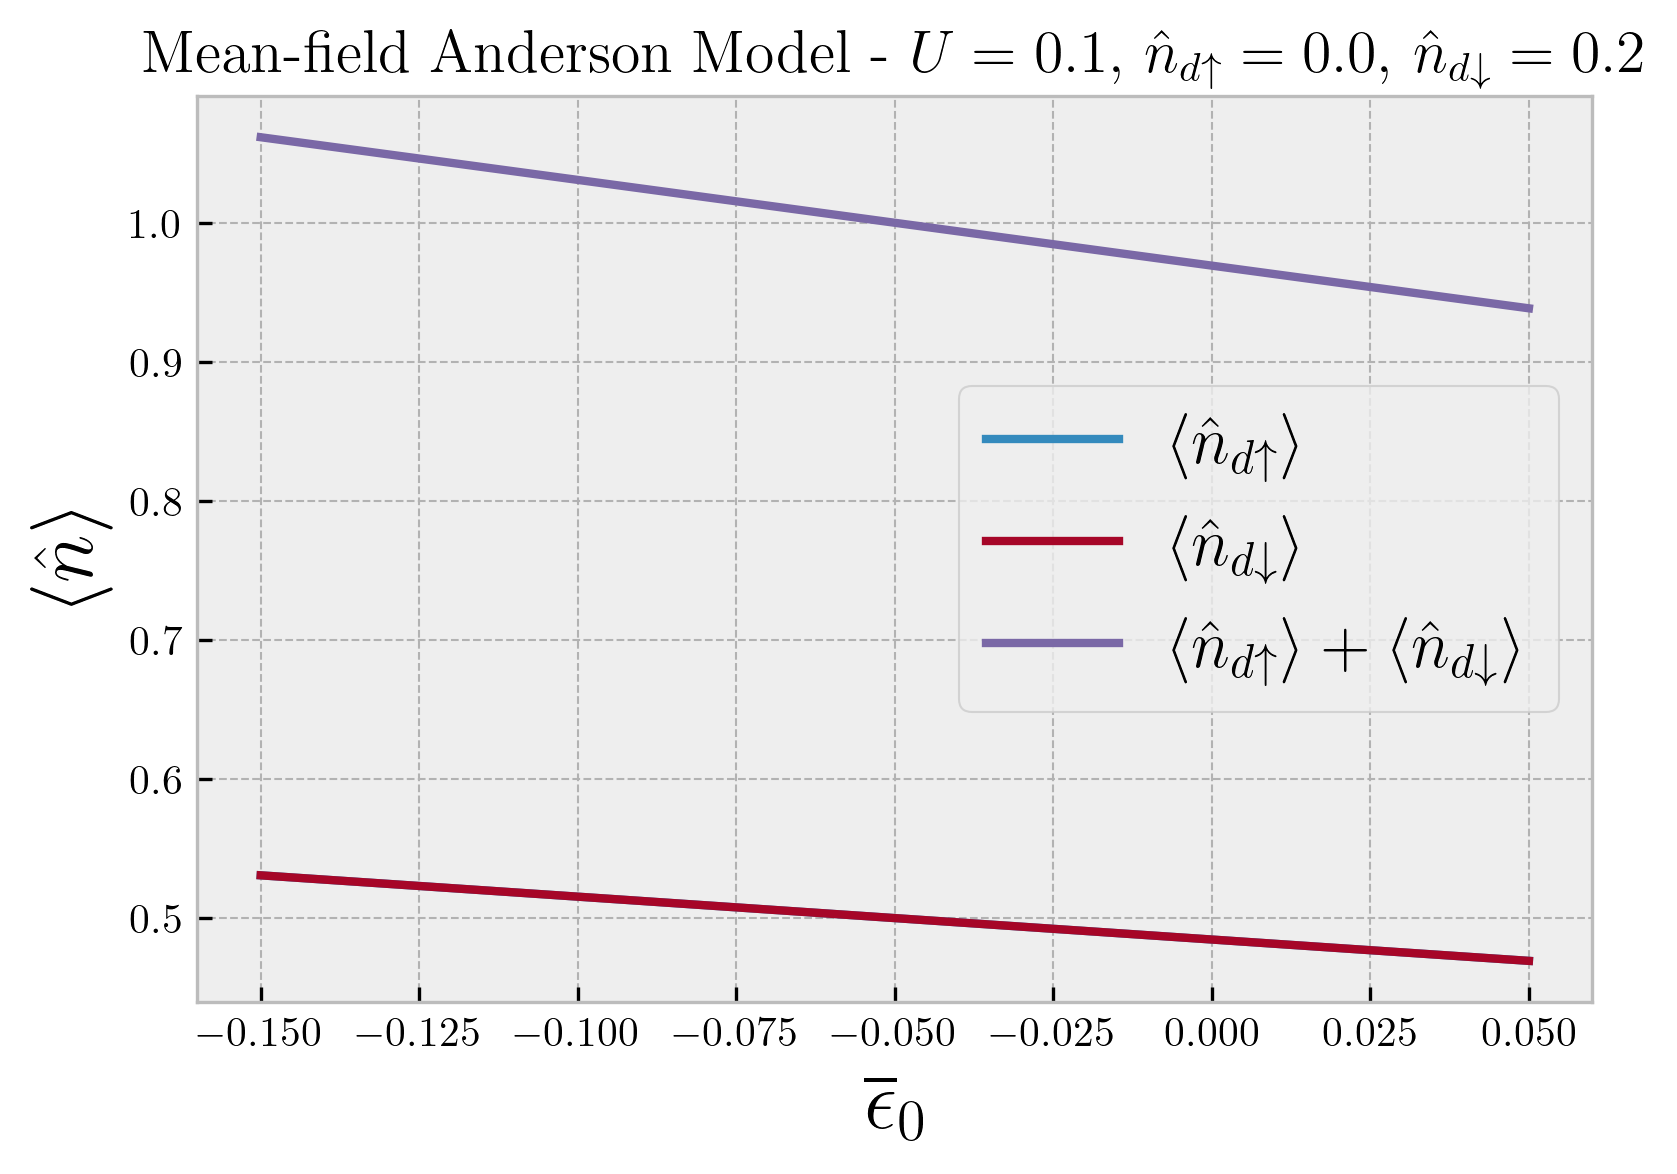
\includegraphics[width=\linewidth]{fig/plot-U_0.1-up_0.0-down_0.2.png}
\end{subfigure}%
\begin{subfigure}{.5\textwidth}
  \centering
  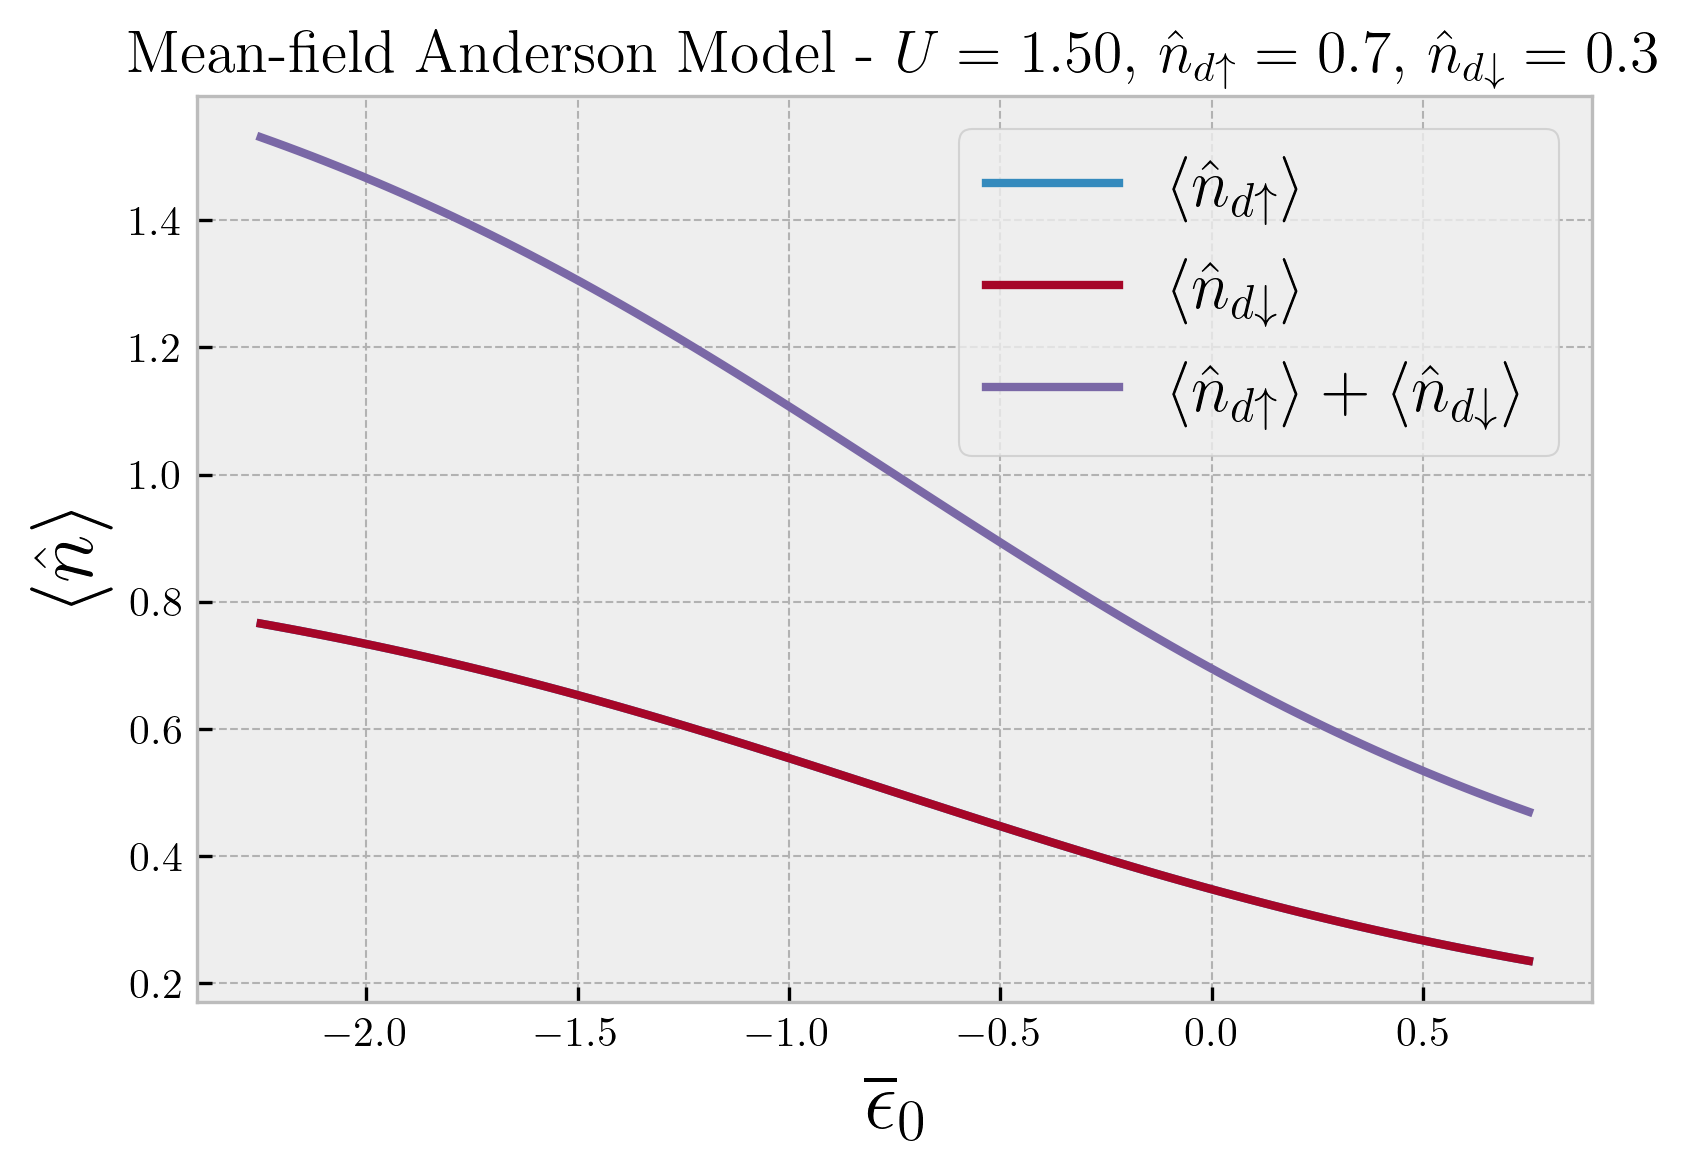
\includegraphics[width=\linewidth]{fig/plot-U_1.5-up_0.7-down_0.3.png}
\end{subfigure}
\end{figure}

\begin{figure}[H]
\centering
\begin{subfigure}{.5\textwidth}
  \centering
  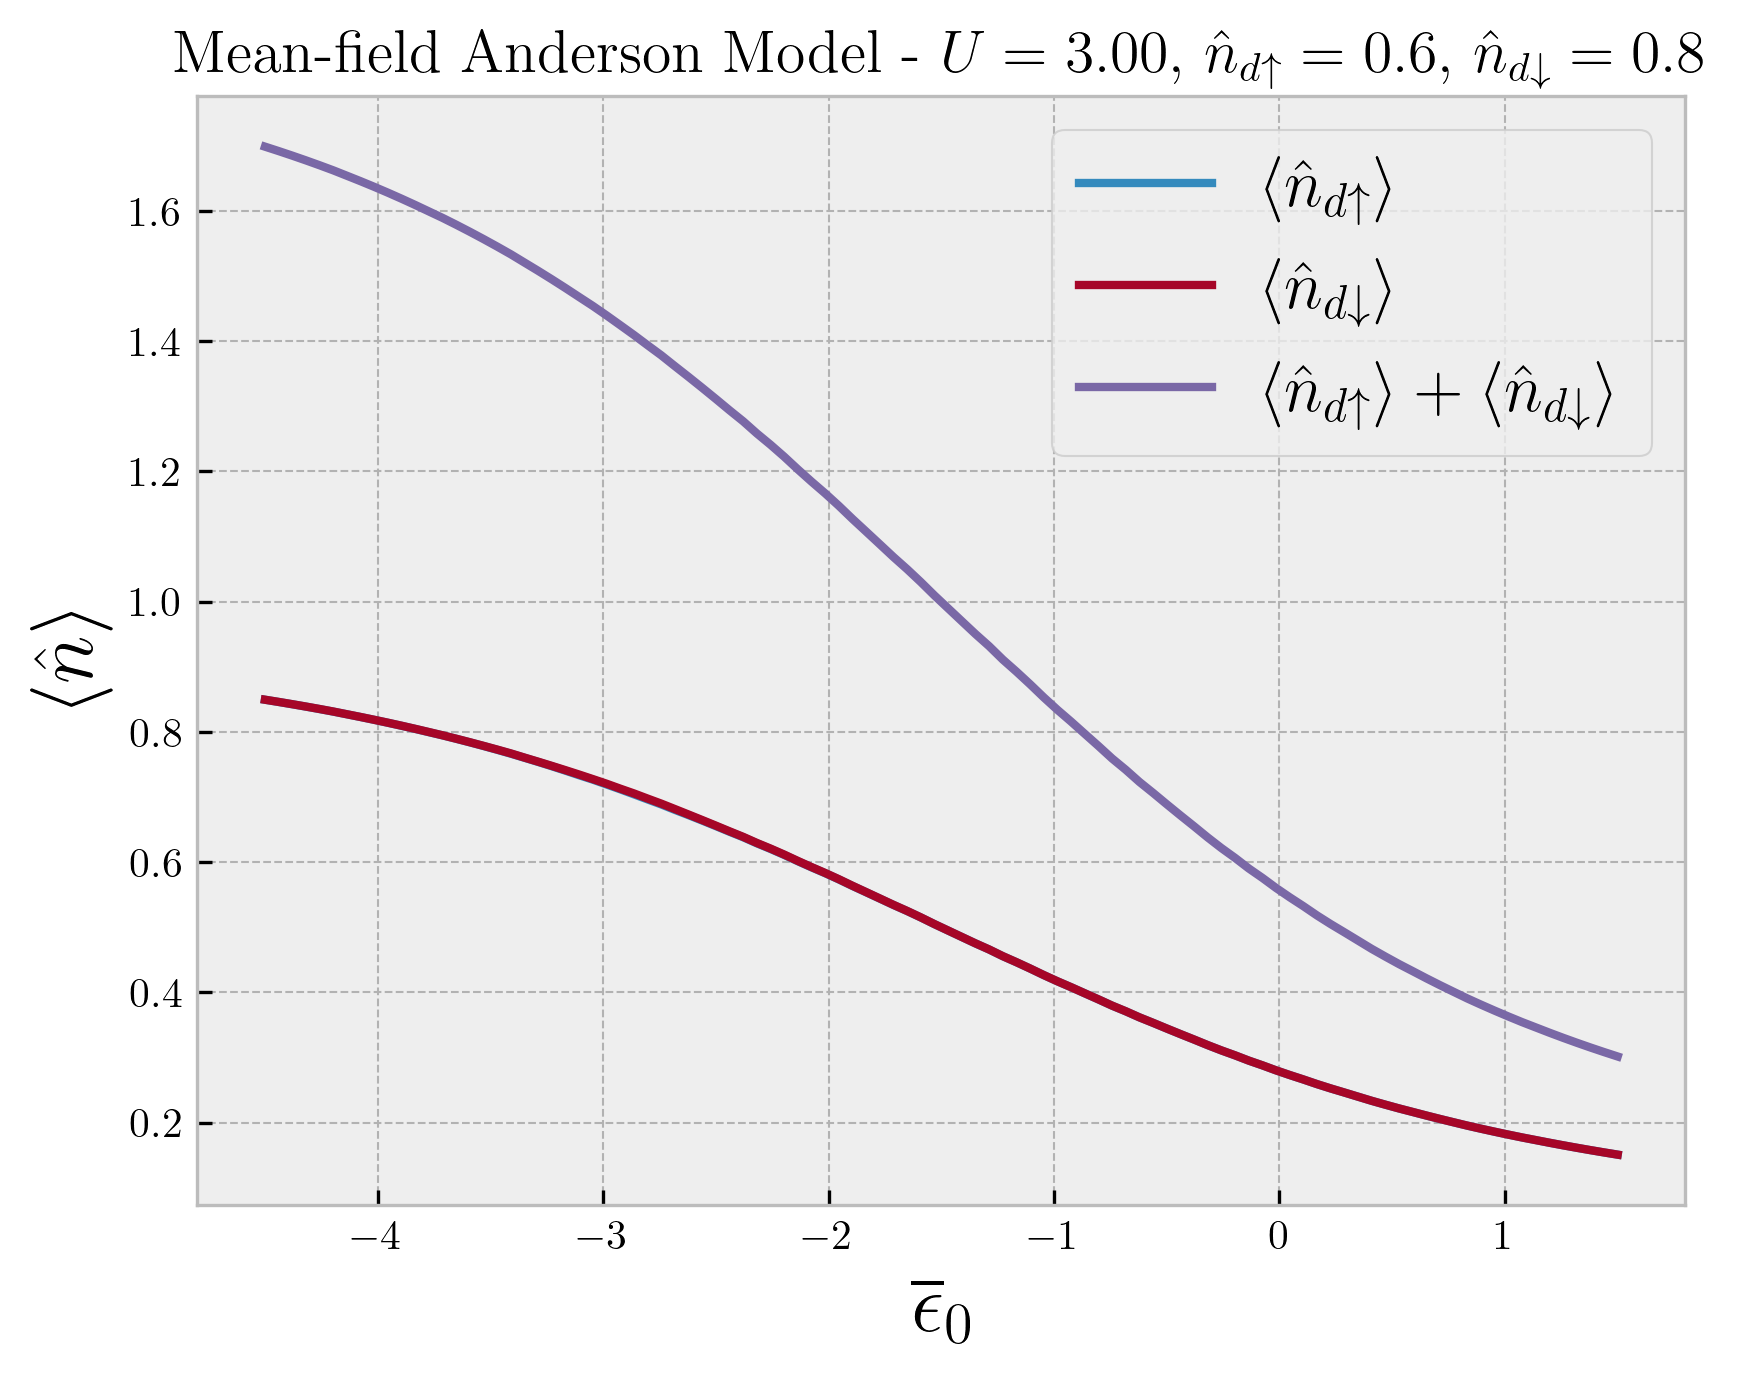
\includegraphics[width=\linewidth]{fig/plot-U_3.0-up_0.6-down_0.8.png}
\end{subfigure}%
\begin{subfigure}{.5\textwidth}
  \centering
  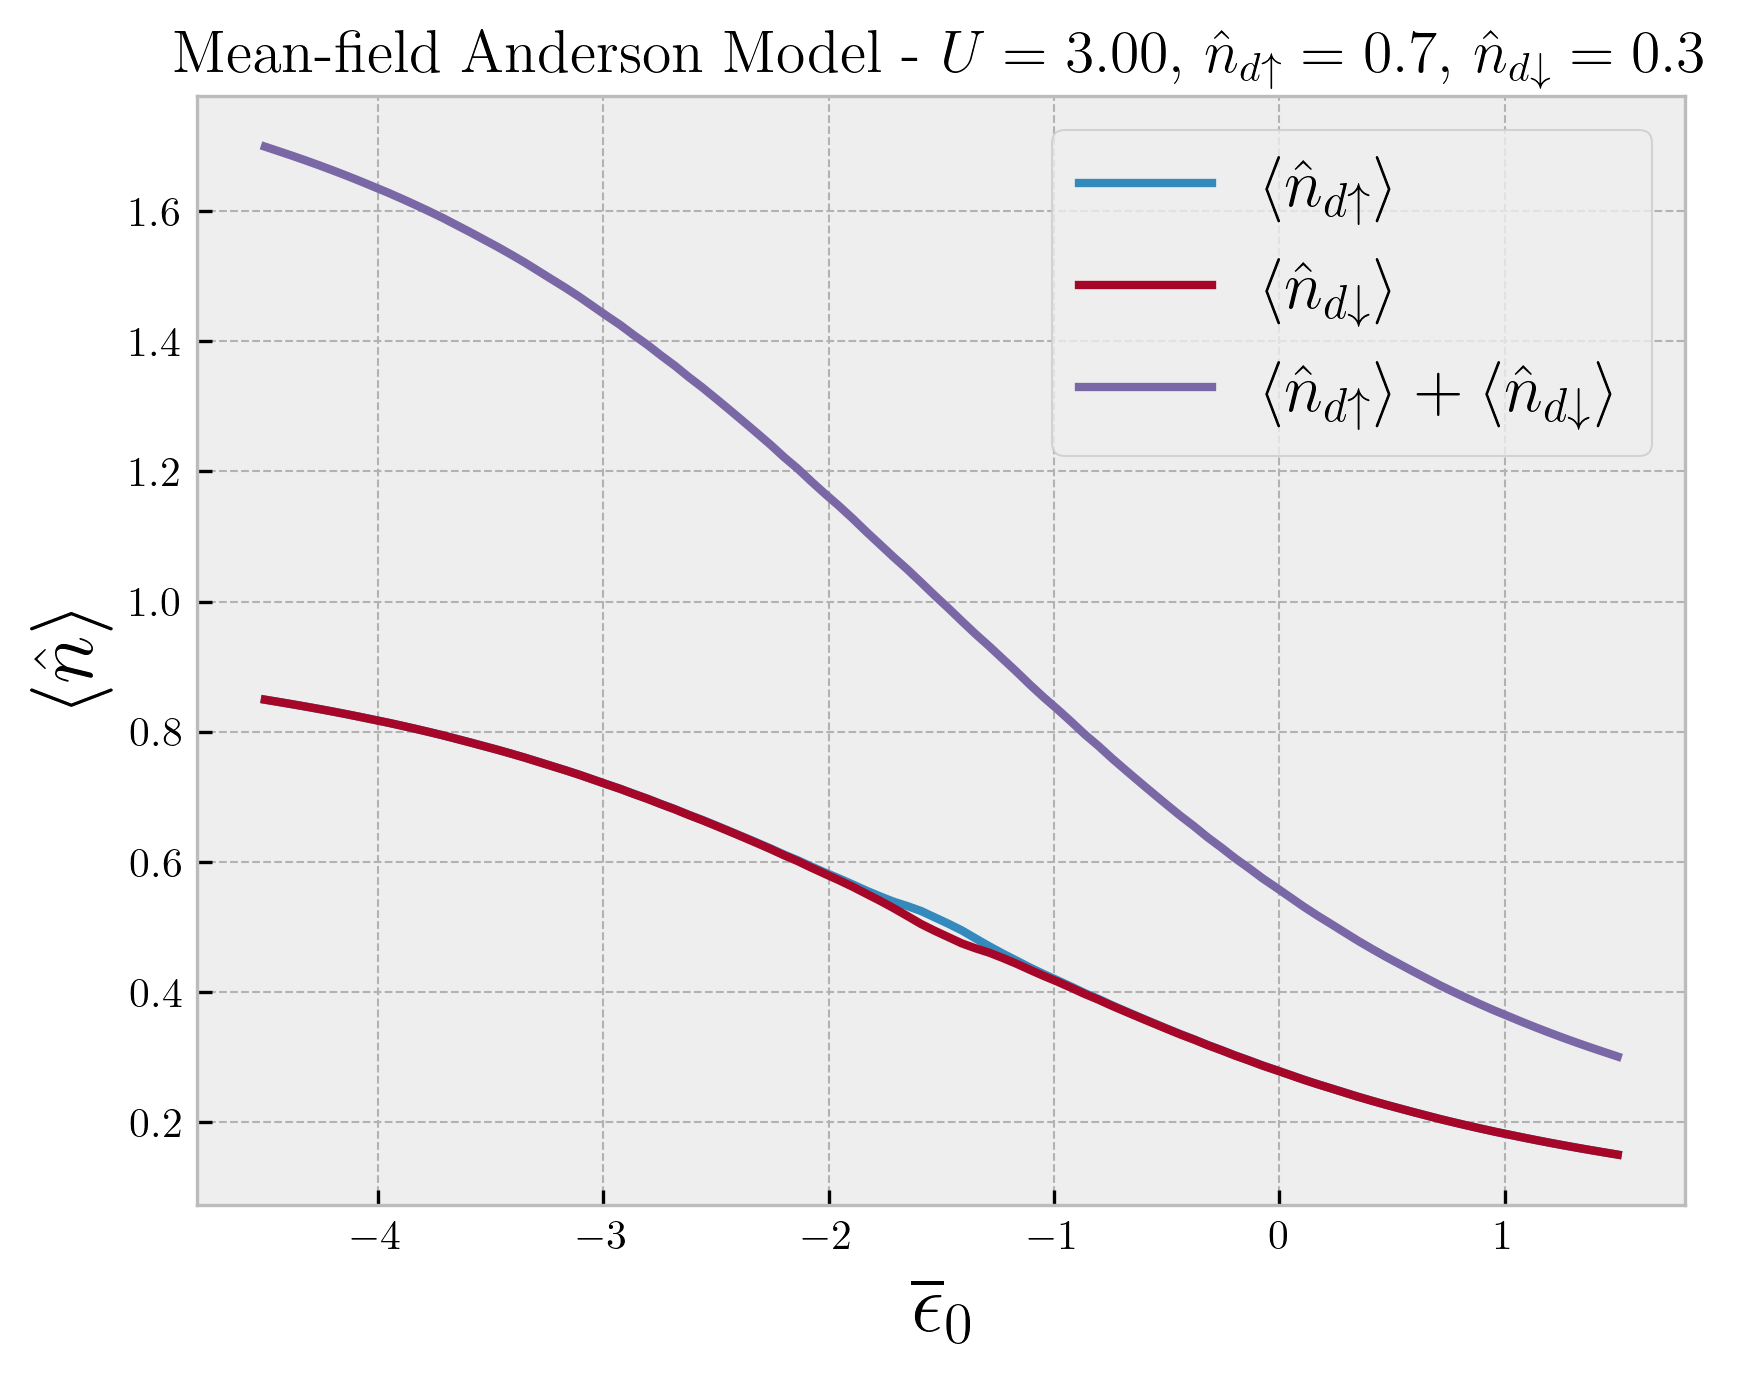
\includegraphics[width=\linewidth]{fig/plot-U_3.0-up_0.7-down_0.3.png}
\end{subfigure}
\end{figure}

\n\n\n\n

\begin{figure}[H]
\centering
\begin{subfigure}{.5\textwidth}
  \centering
  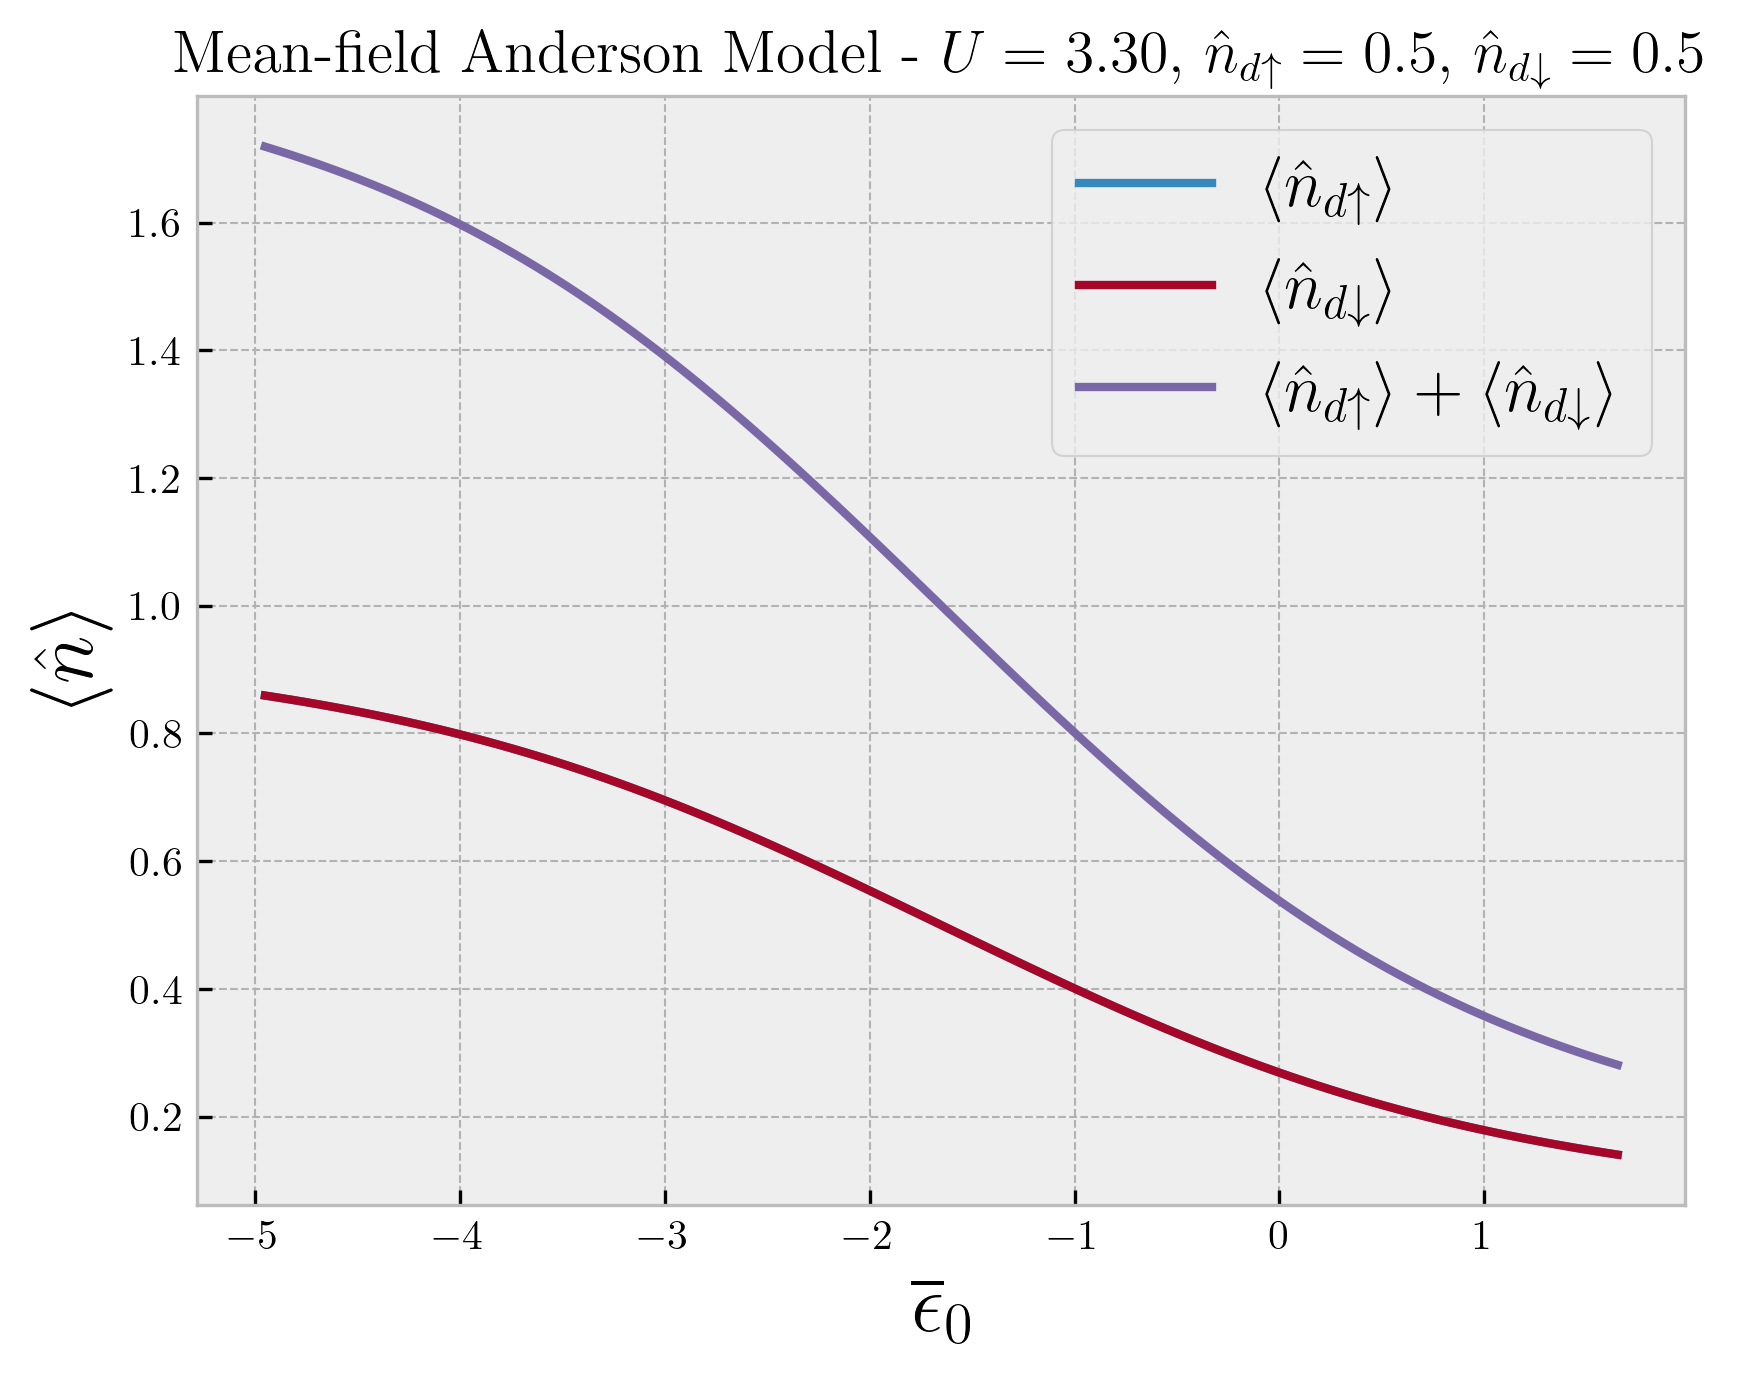
\includegraphics[width=\linewidth]{fig/plot-U_3.3-up_0.5-down_0.5.png}
\end{subfigure}%
\begin{subfigure}{.5\textwidth}
  \centering
  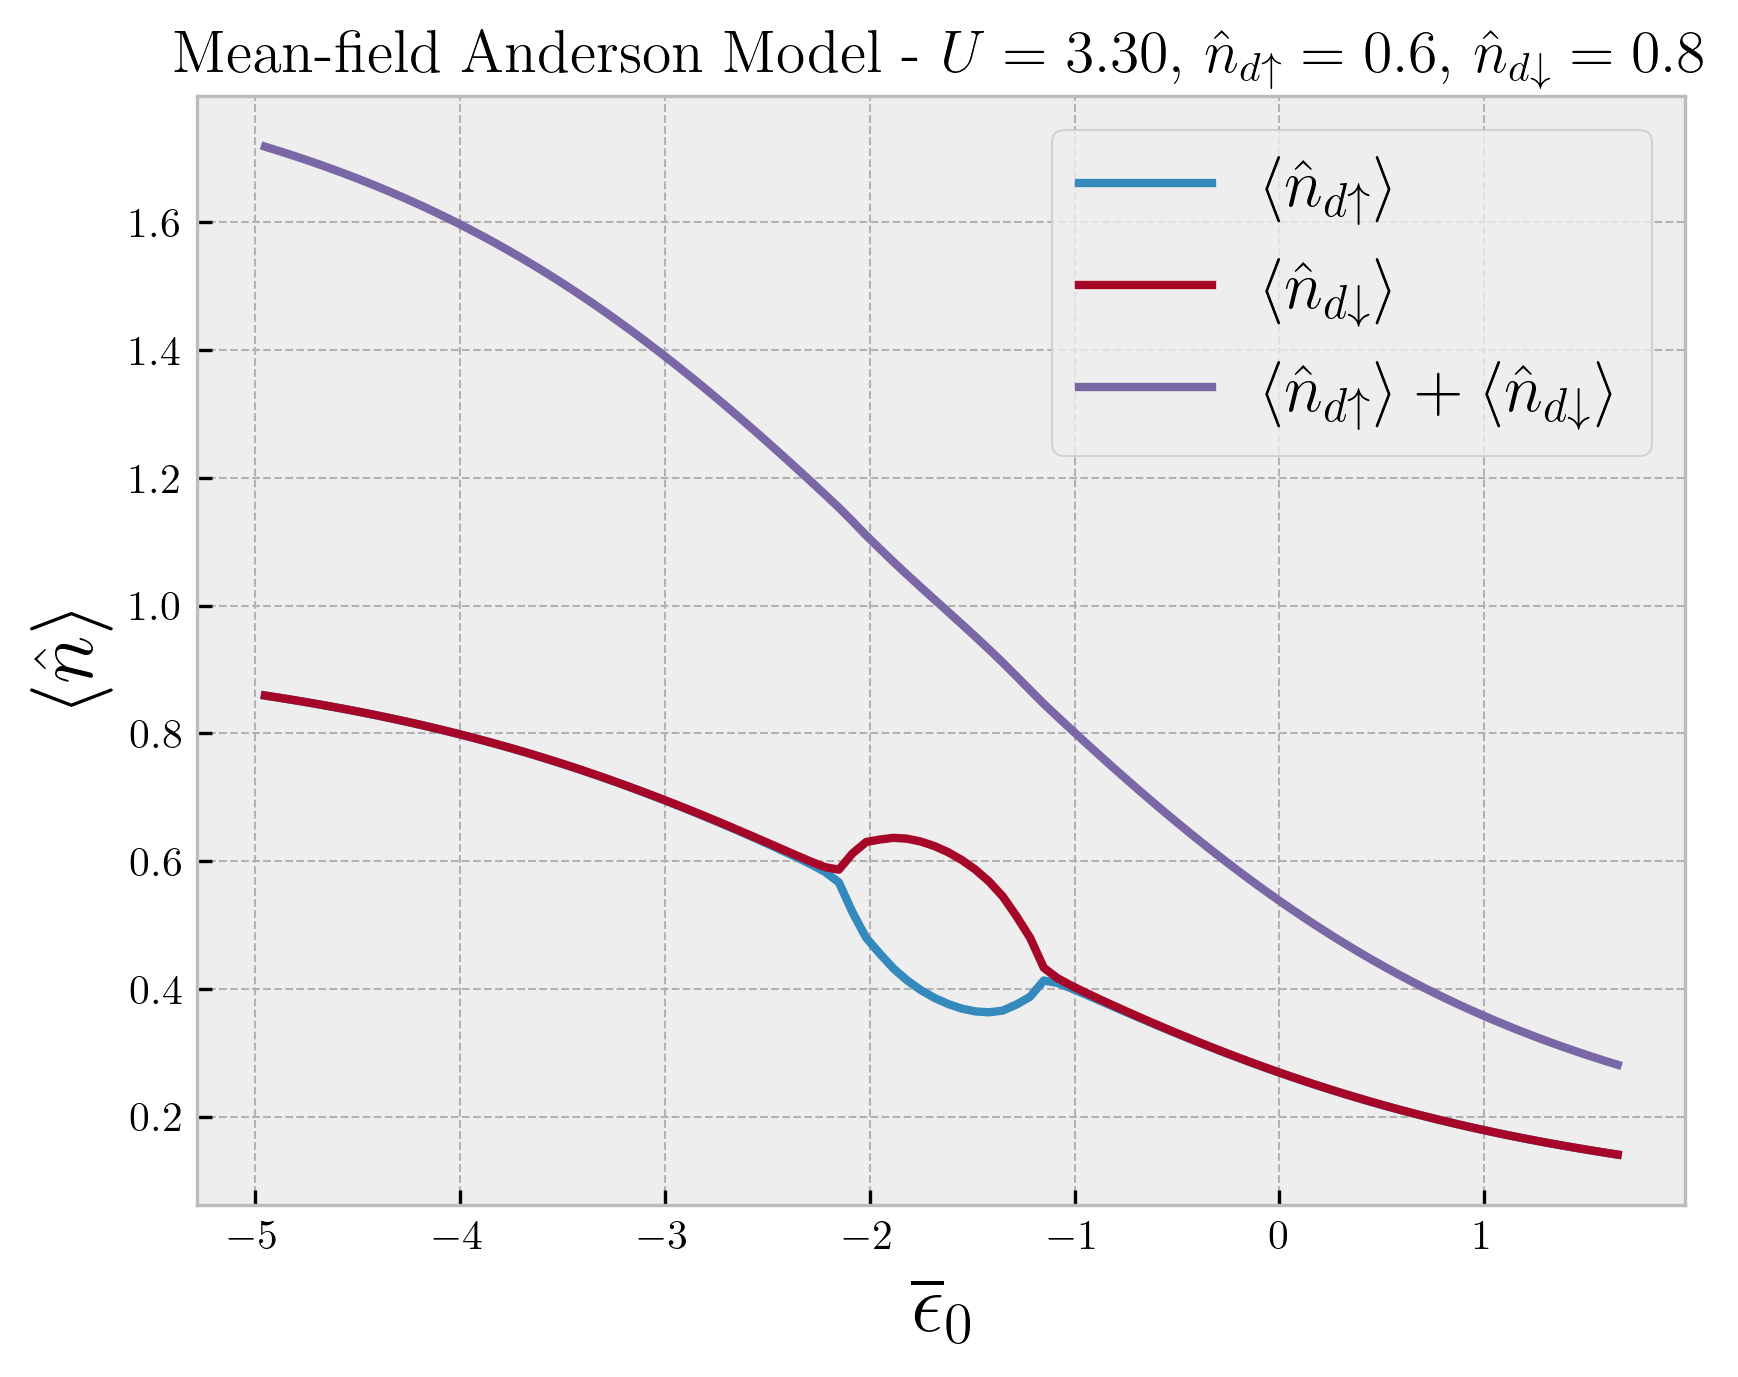
\includegraphics[width=\linewidth]{fig/plot-U_3.3-up_0.6-down_0.8.png}
\end{subfigure}
\end{figure}

\n\n\n\n

\begin{figure}[H]
\centering
\begin{subfigure}{.5\textwidth}
  \centering
  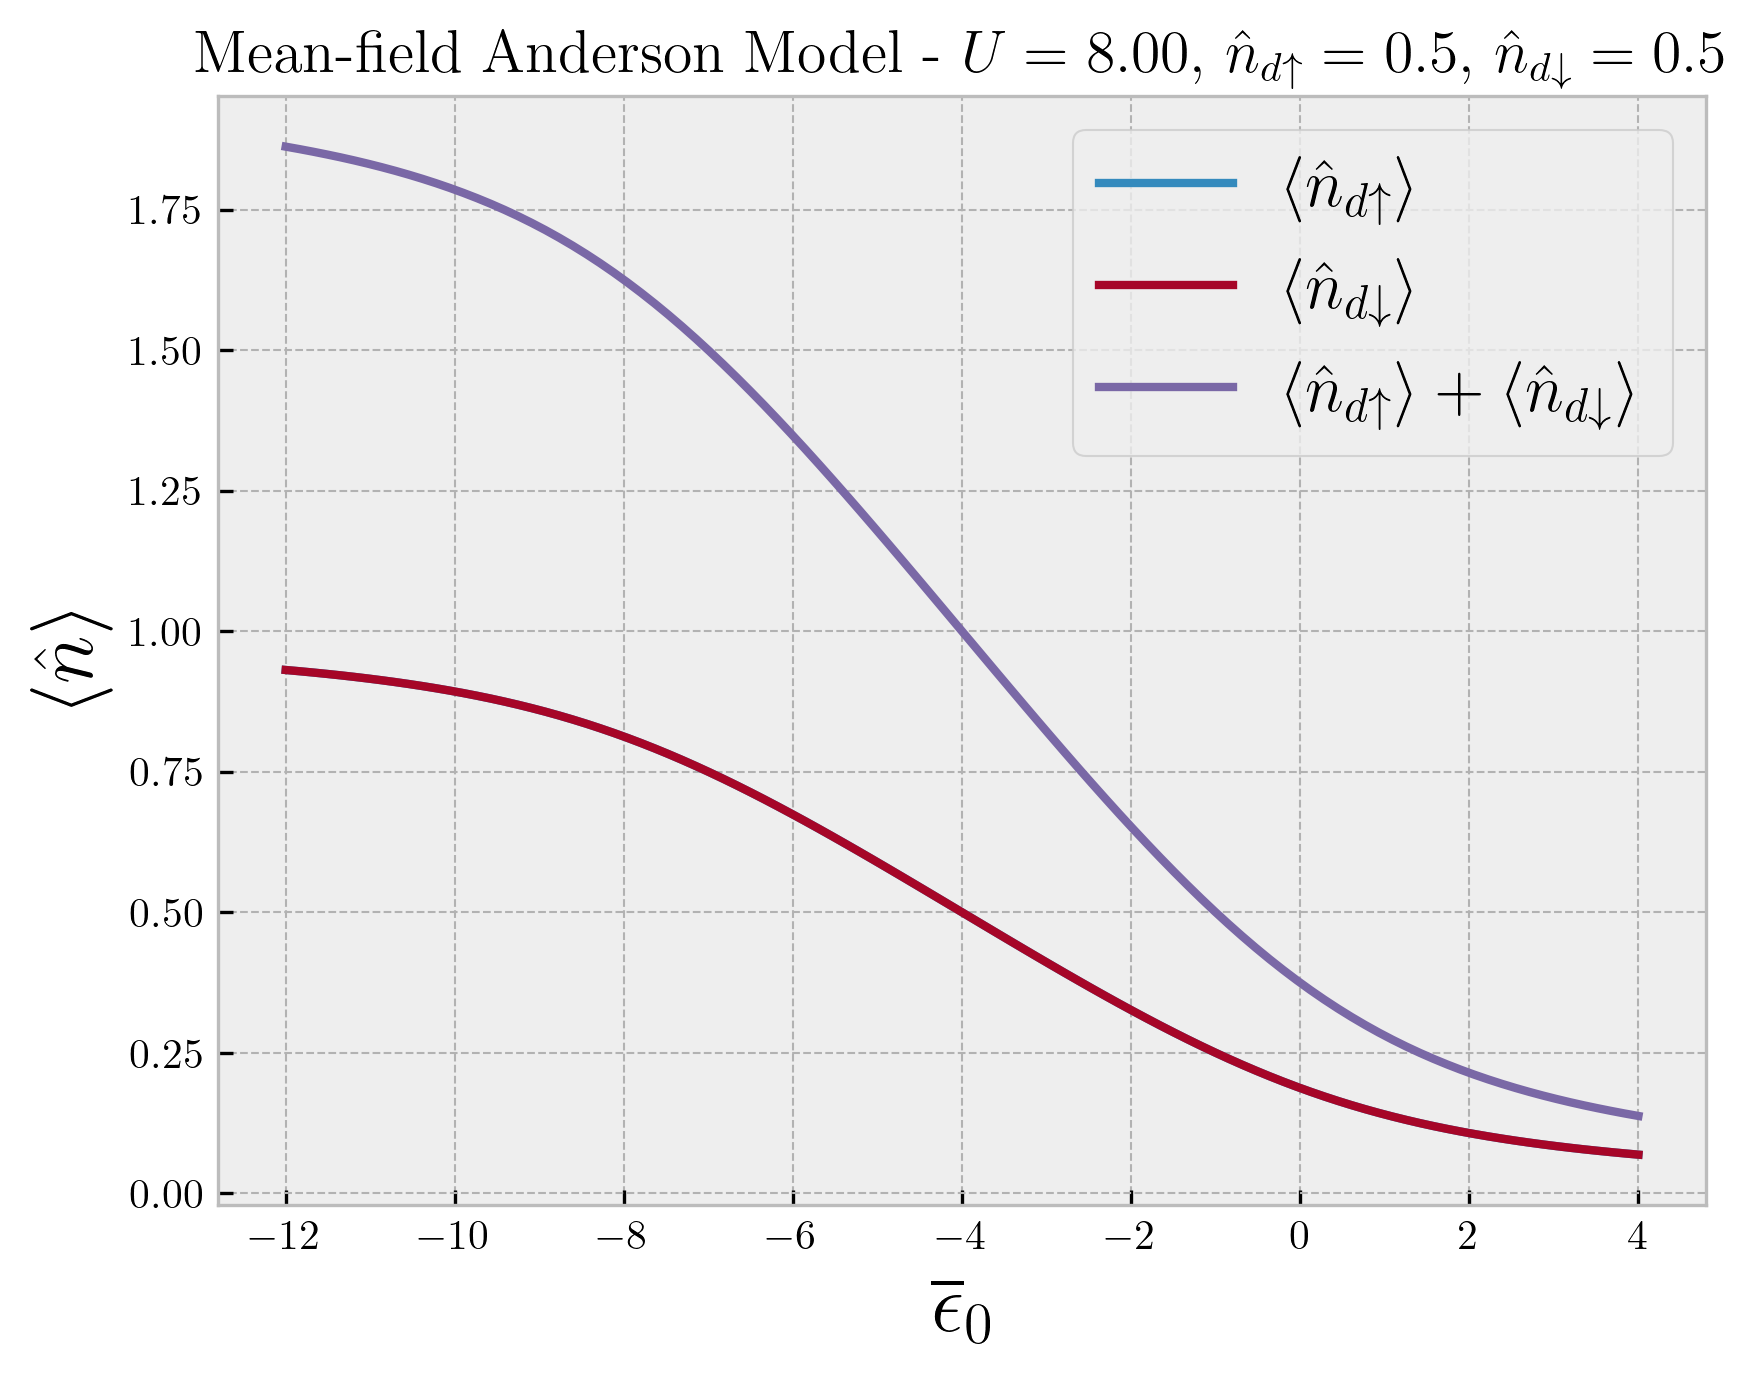
\includegraphics[width=\linewidth]{fig/plot-U_8.0-up_0.5-down_0.5.png}
\end{subfigure}%
\begin{subfigure}{.5\textwidth}
  \centering
  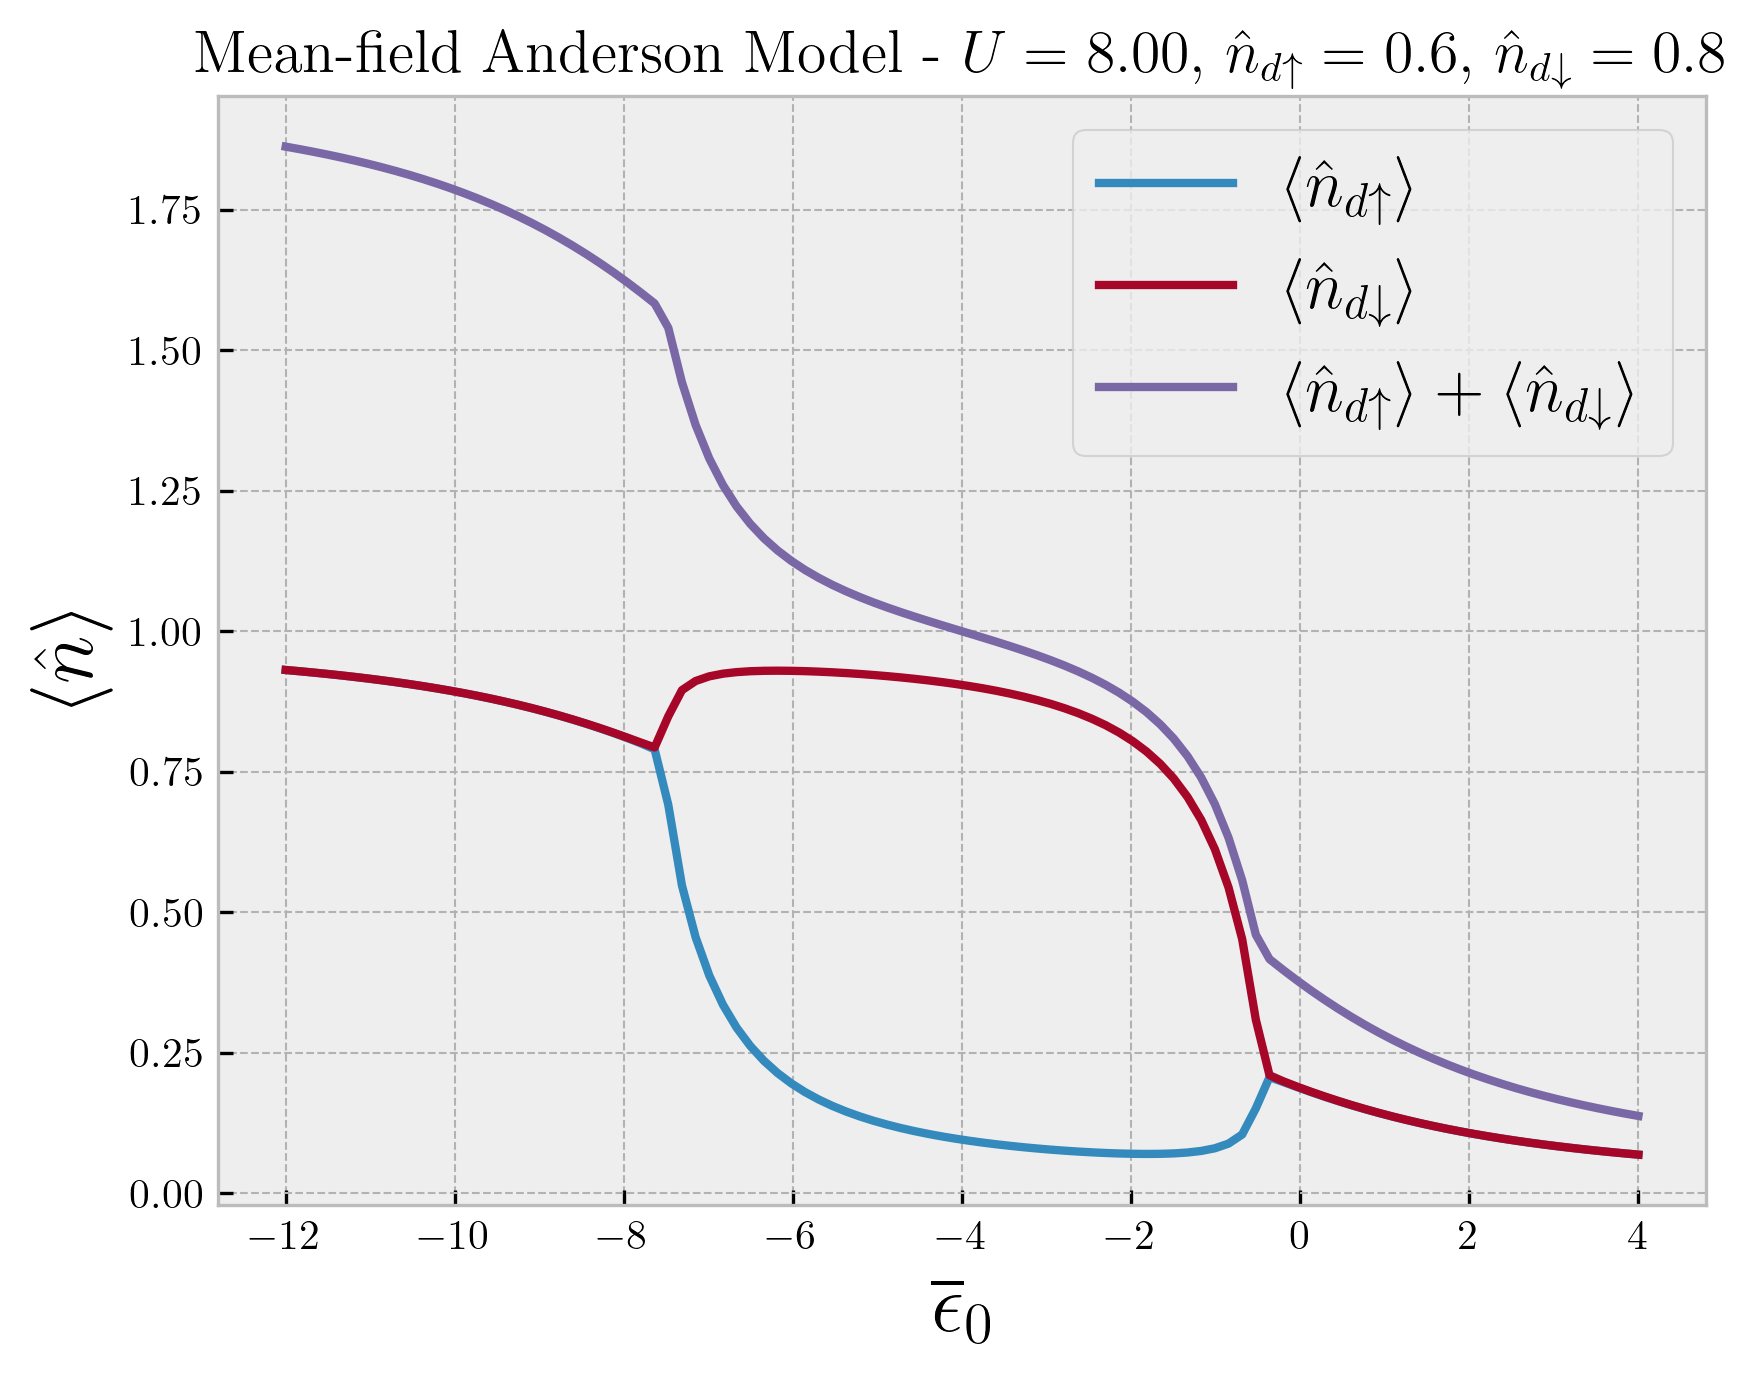
\includegraphics[width=\linewidth]{fig/plot-U_8.0-up_0.6-down_0.8.png}
\end{subfigure}
\end{figure}

\begin{figure}[H]
\centering
\begin{subfigure}{.5\textwidth}
  \centering
  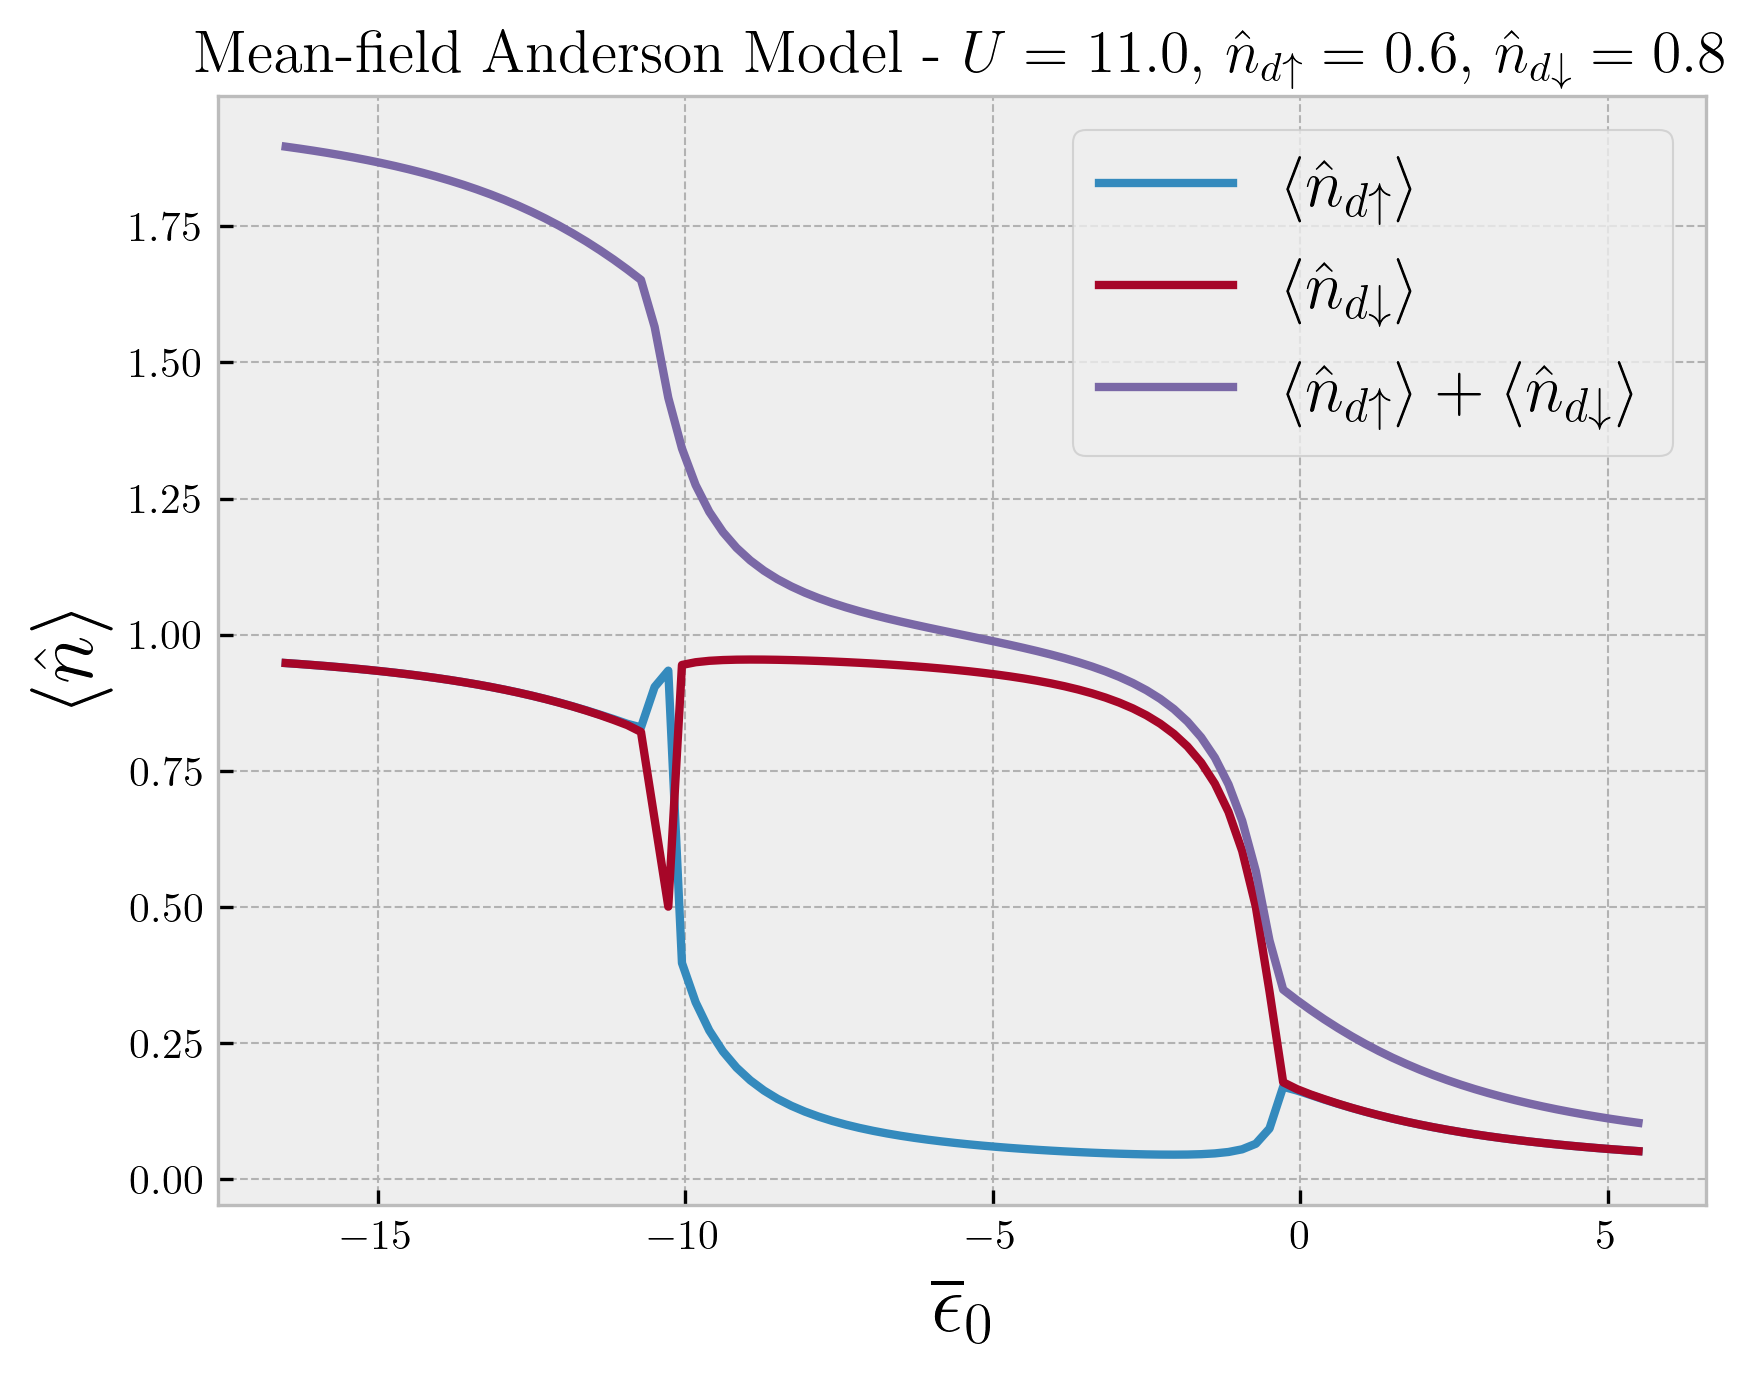
\includegraphics[width=\linewidth]{fig/plot-U_11-up_0.6-down_0.8.png}
\end{subfigure}%
\begin{subfigure}{.5\textwidth}
  \centering
  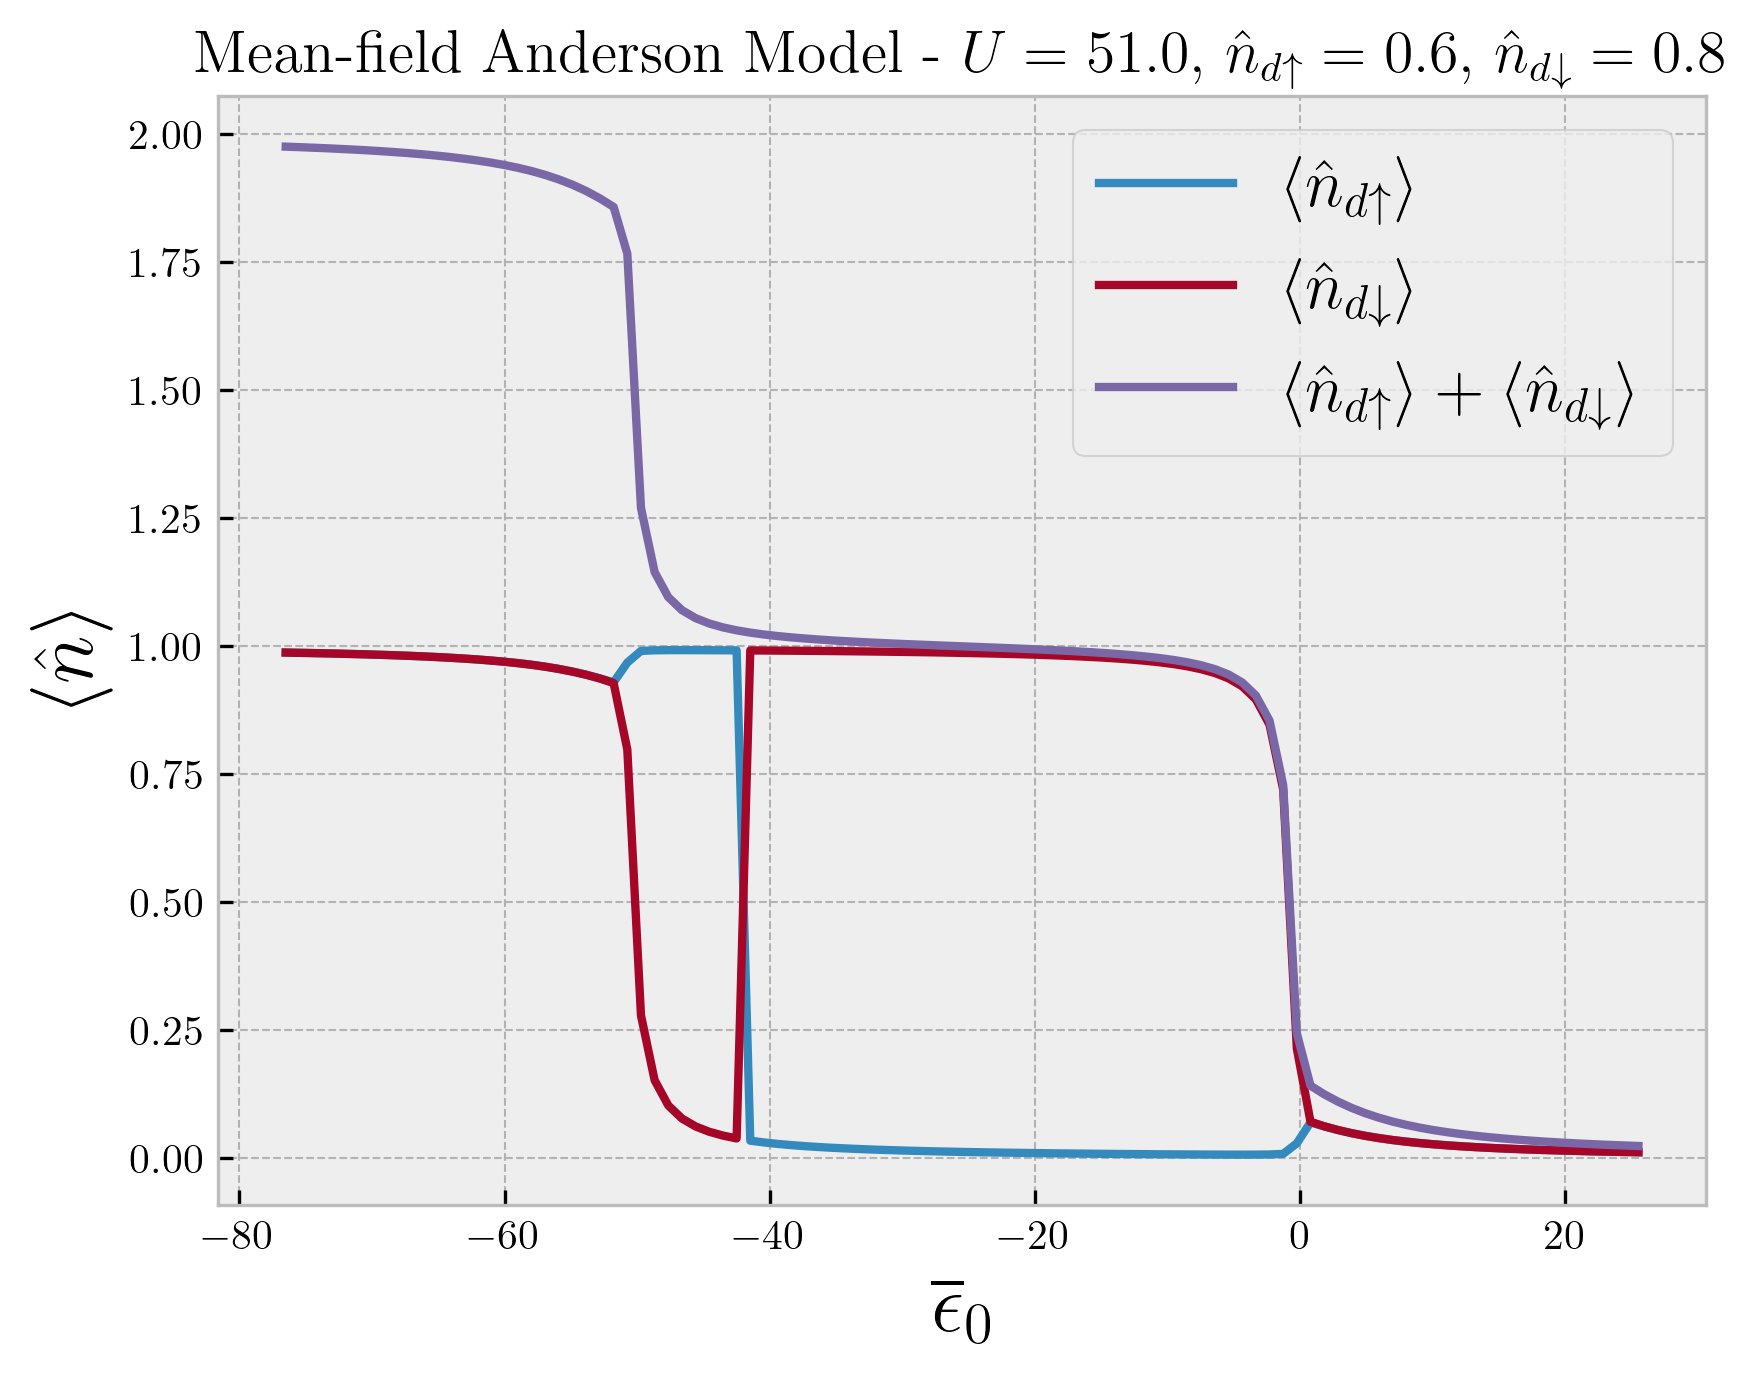
\includegraphics[width=\linewidth]{fig/plot-U_51-up_0.6-down_0.8.png}
\end{subfigure}
\end{figure}

\n\n\n\n

\begin{figure}[H]
\centering
\begin{subfigure}{.5\textwidth}
  \centering
  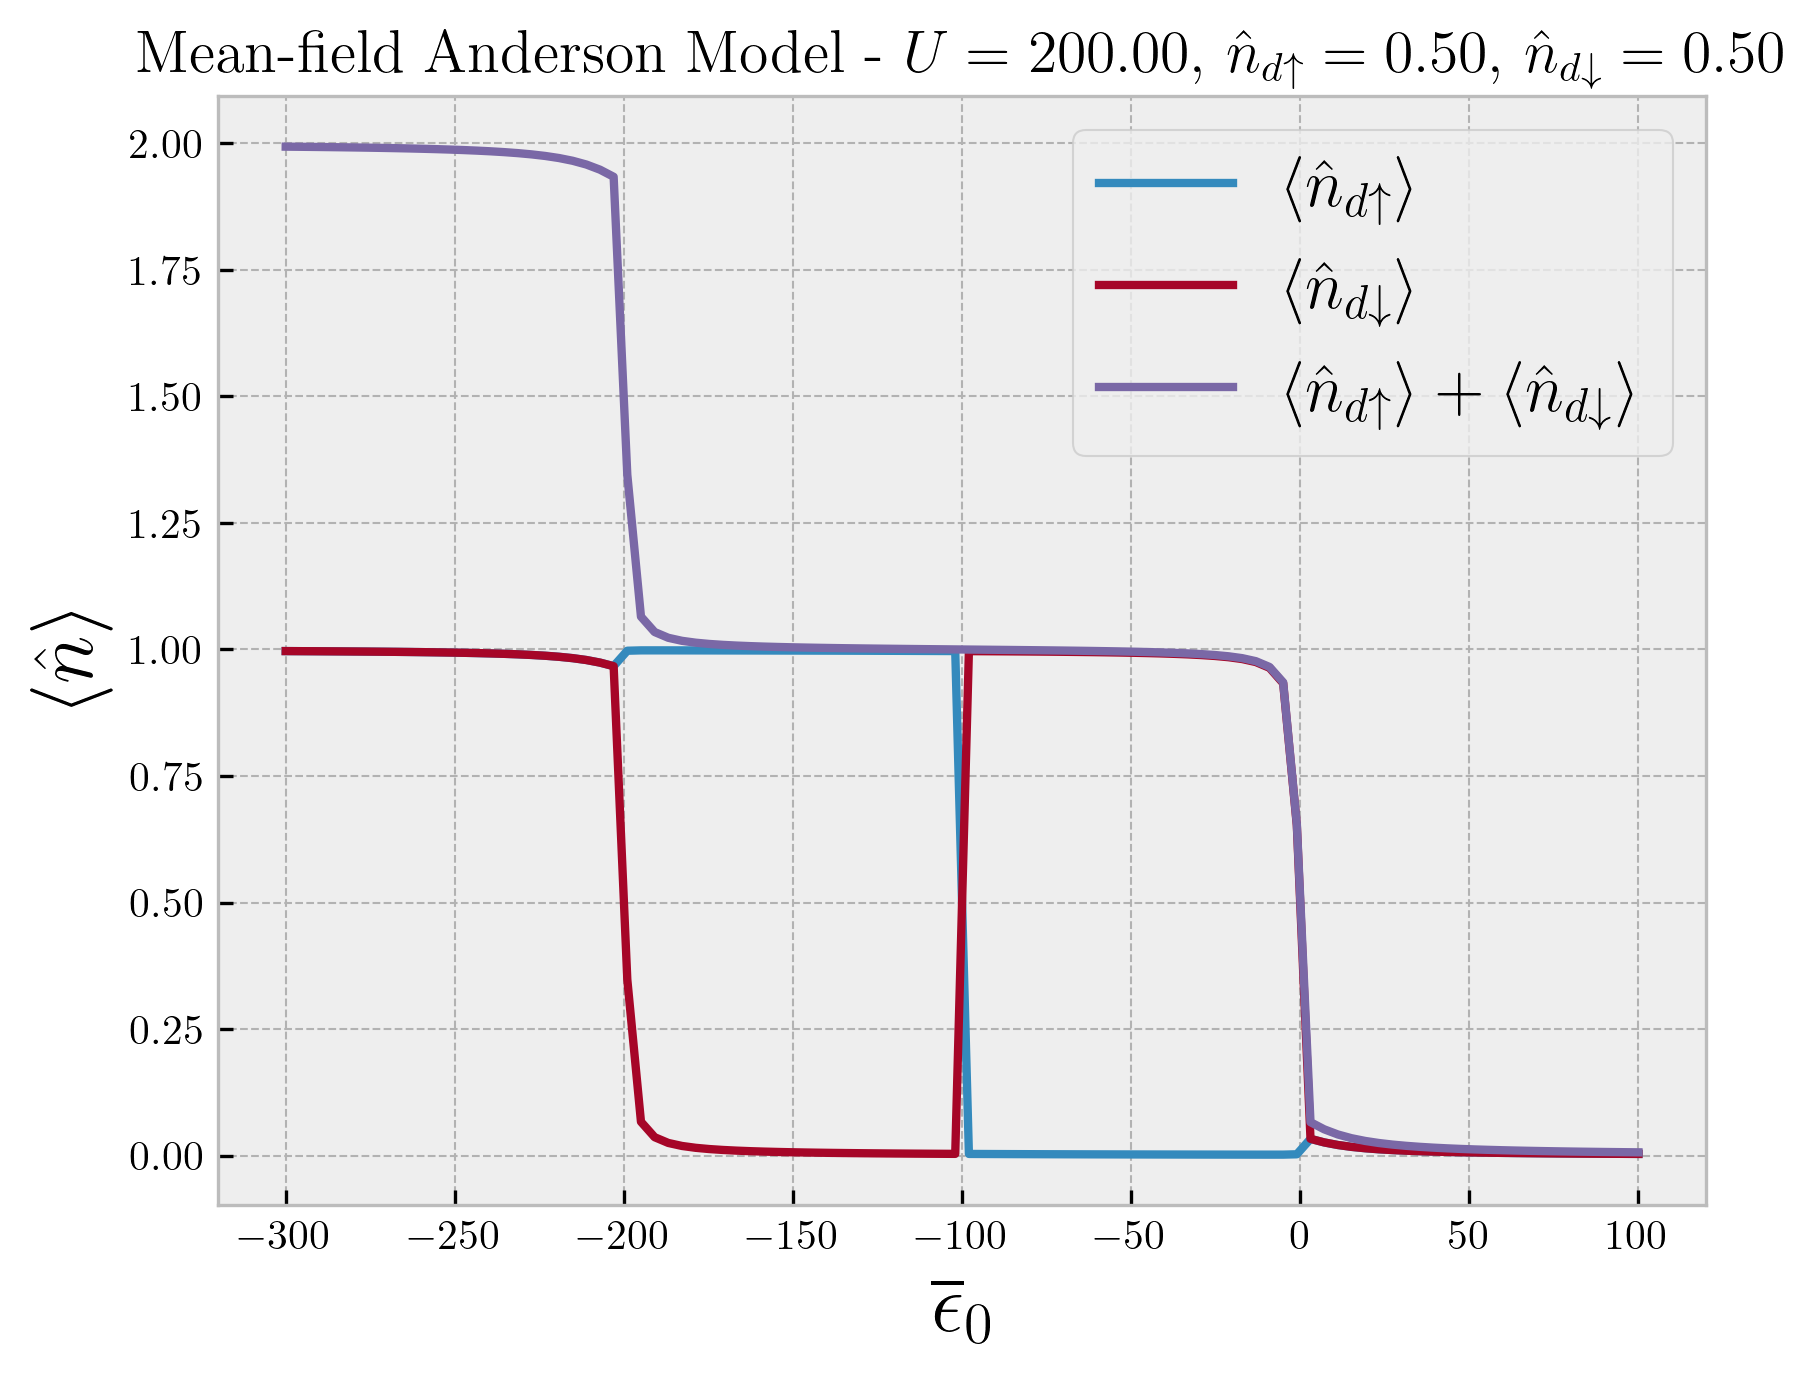
\includegraphics[width=\linewidth]{fig/plot-U_200-up_0.5-down_0.50.png}
\end{subfigure}%
\begin{subfigure}{.5\textwidth}
  \centering
  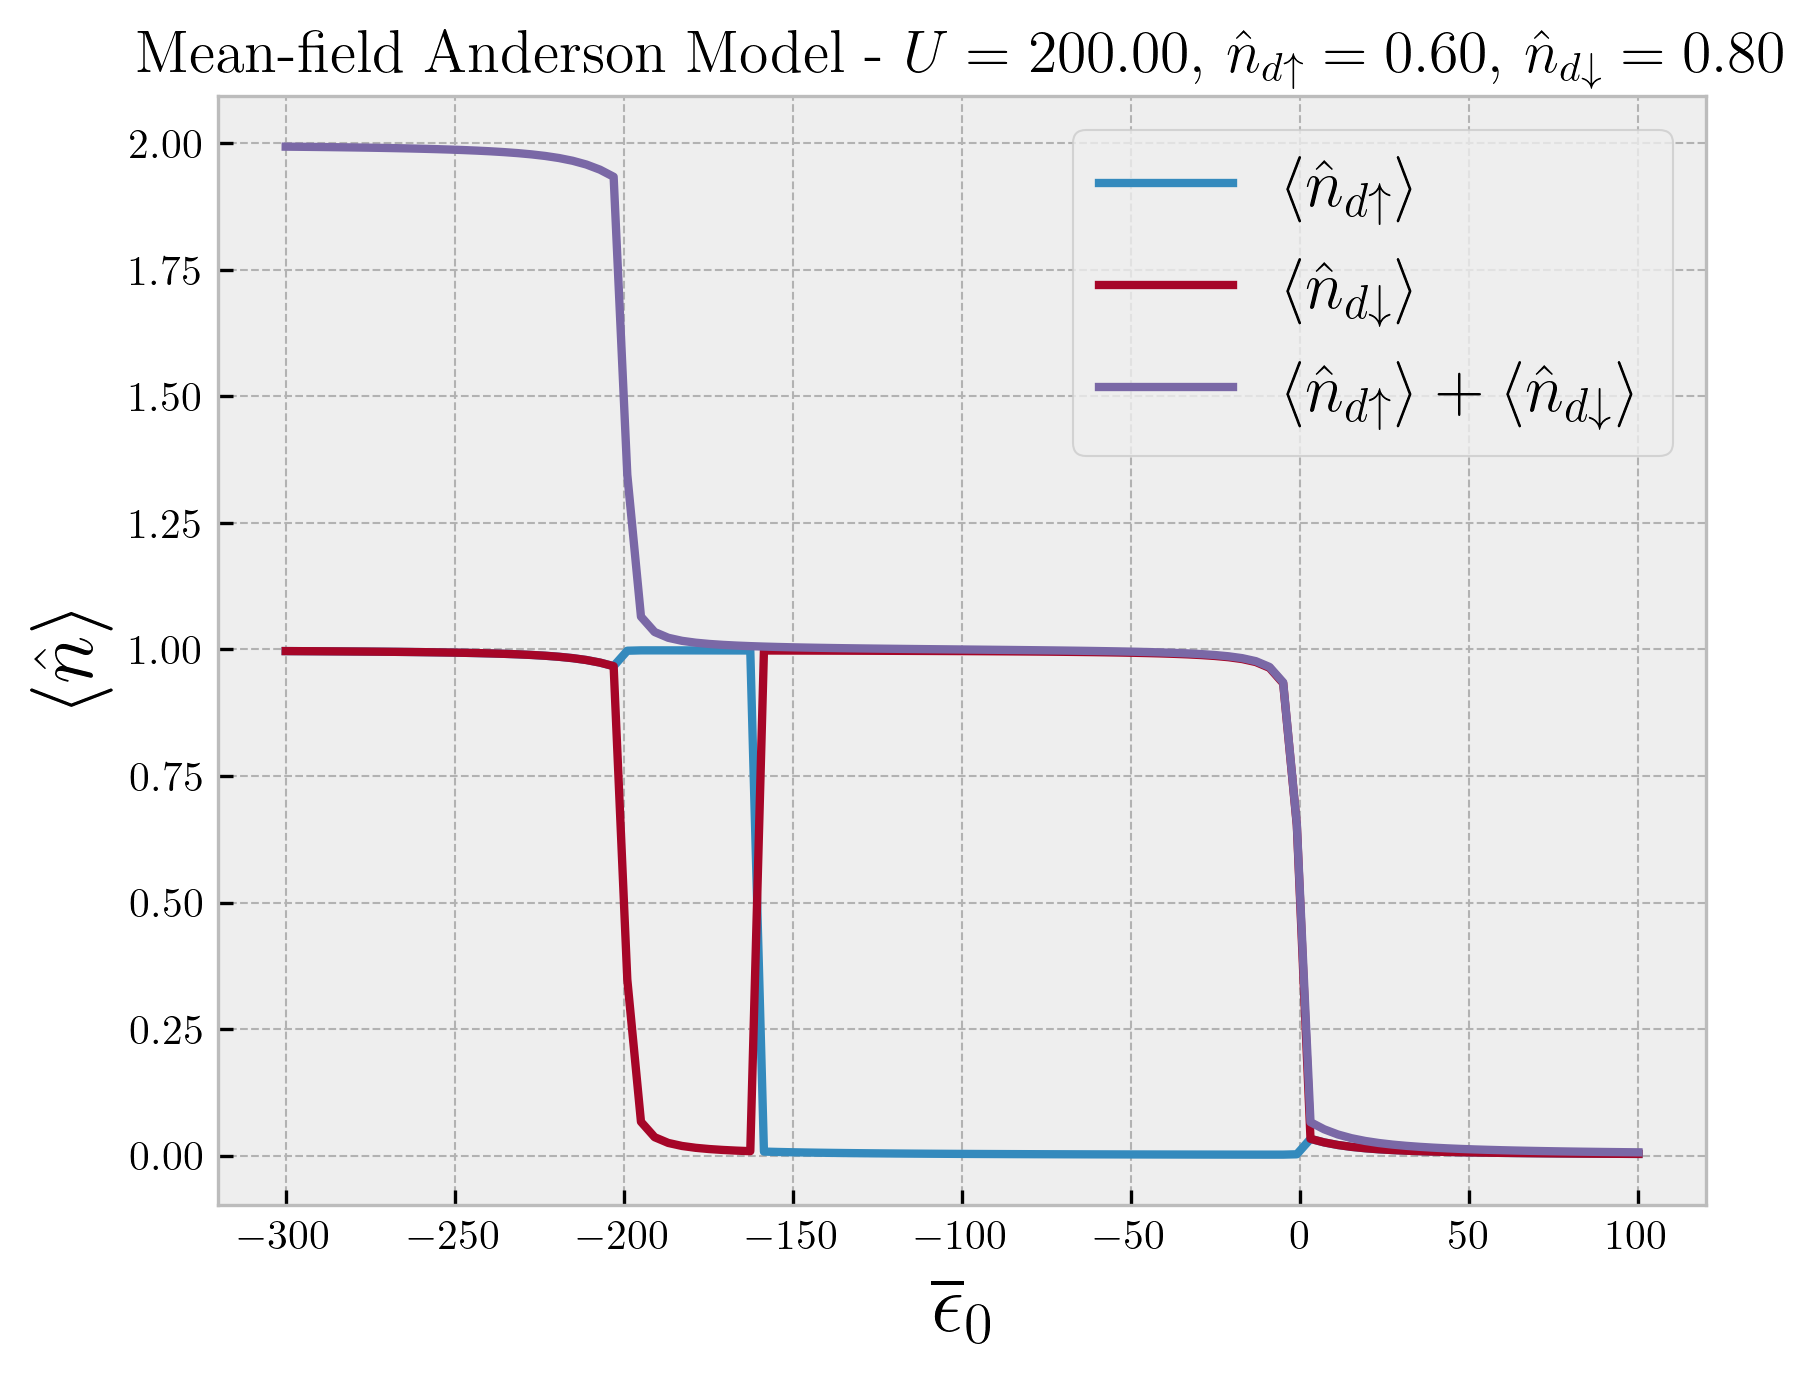
\includegraphics[width=\linewidth]{fig/plot-U_200-up_0.6-down_0.80.png}
\end{subfigure}
\end{figure}

\n\n\n\n

\begin{figure}[H]
\centering
\begin{subfigure}{.5\textwidth}
  \centering
  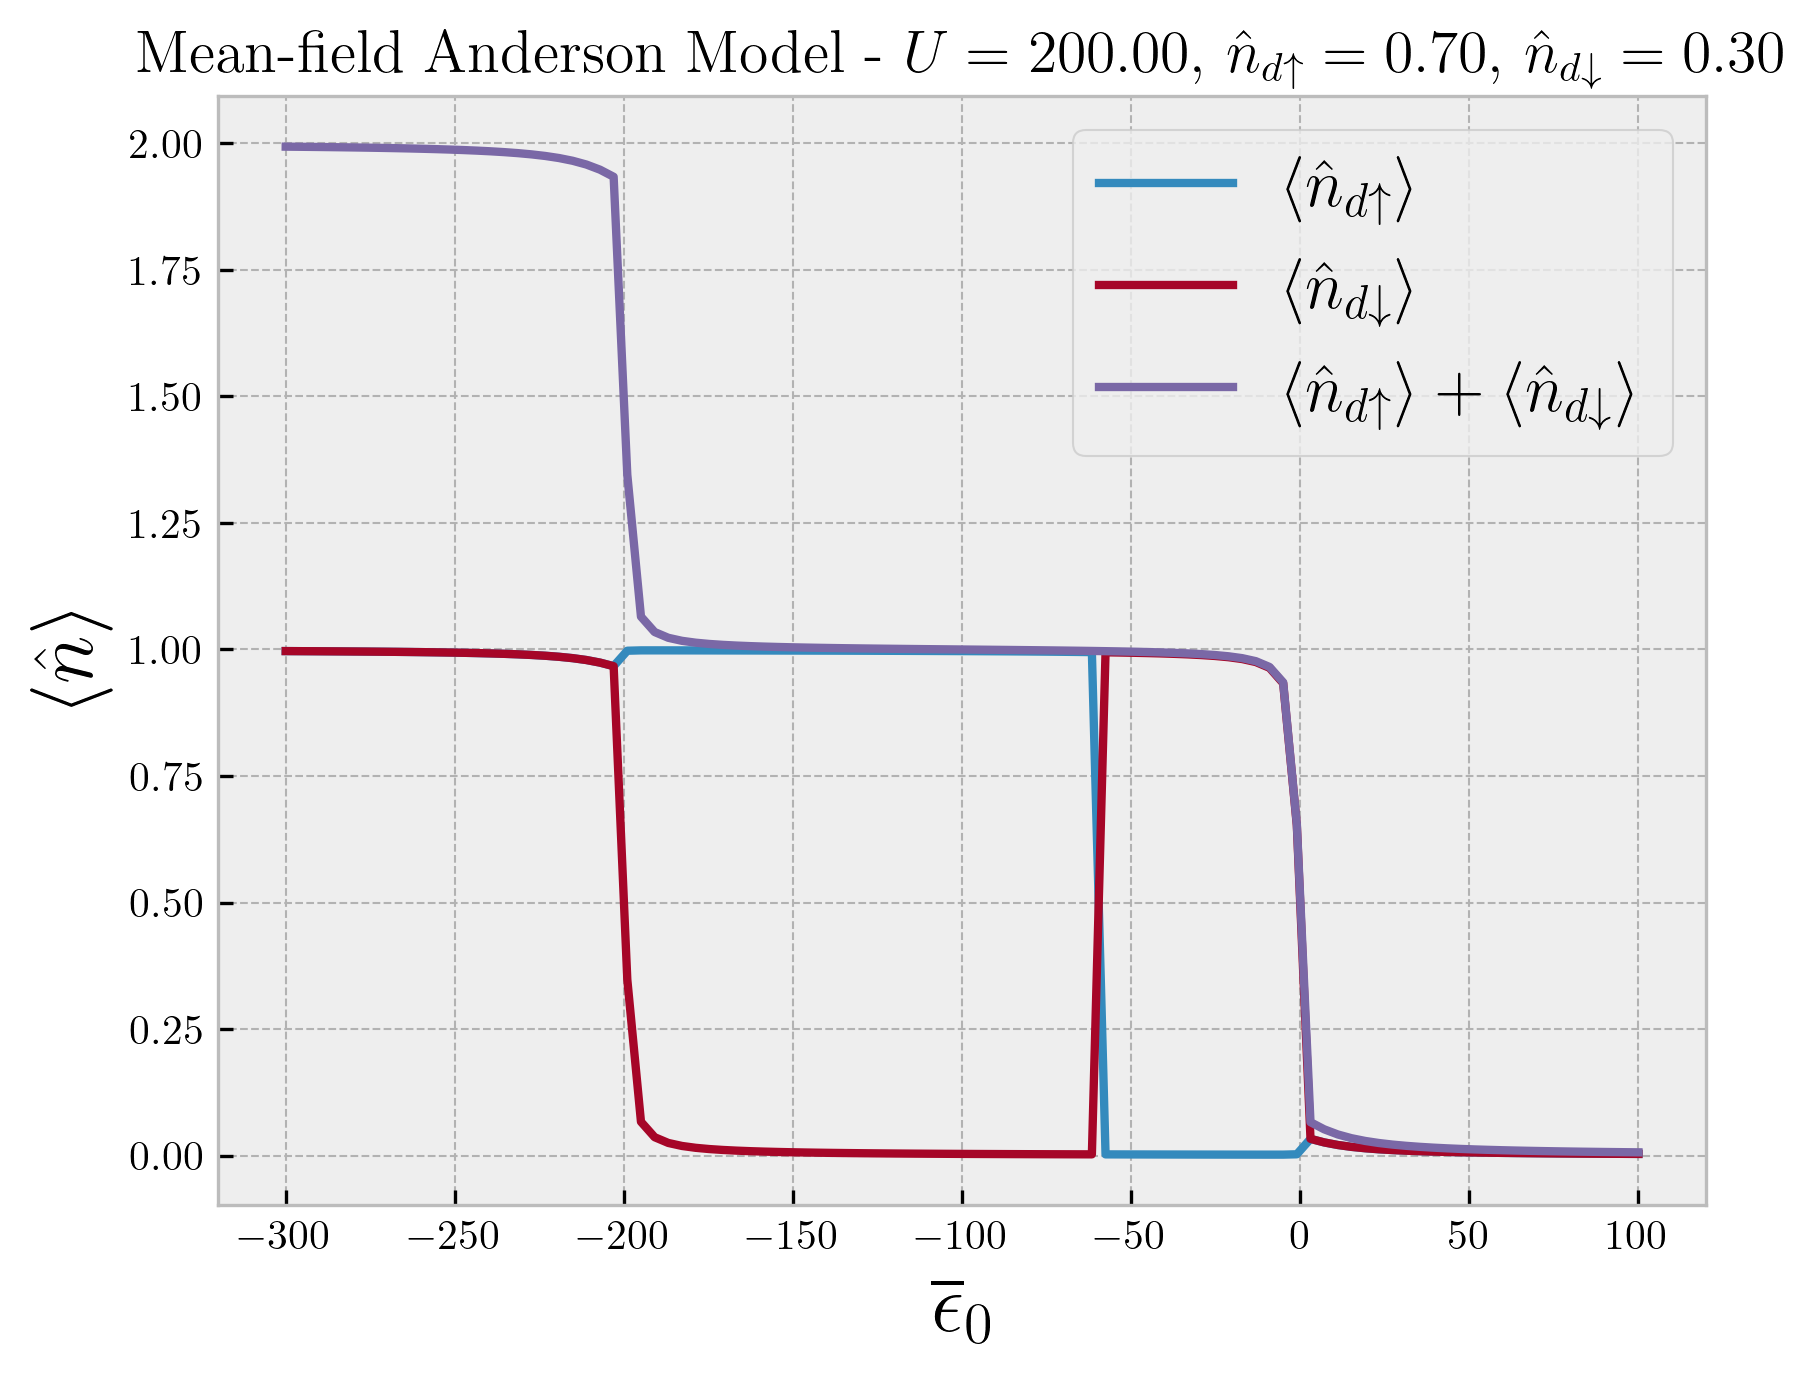
\includegraphics[width=\linewidth]{fig/plot-U_200-up_0.7-down_0.30.png}
\end{subfigure}%
\begin{subfigure}{.5\textwidth}
  \centering
  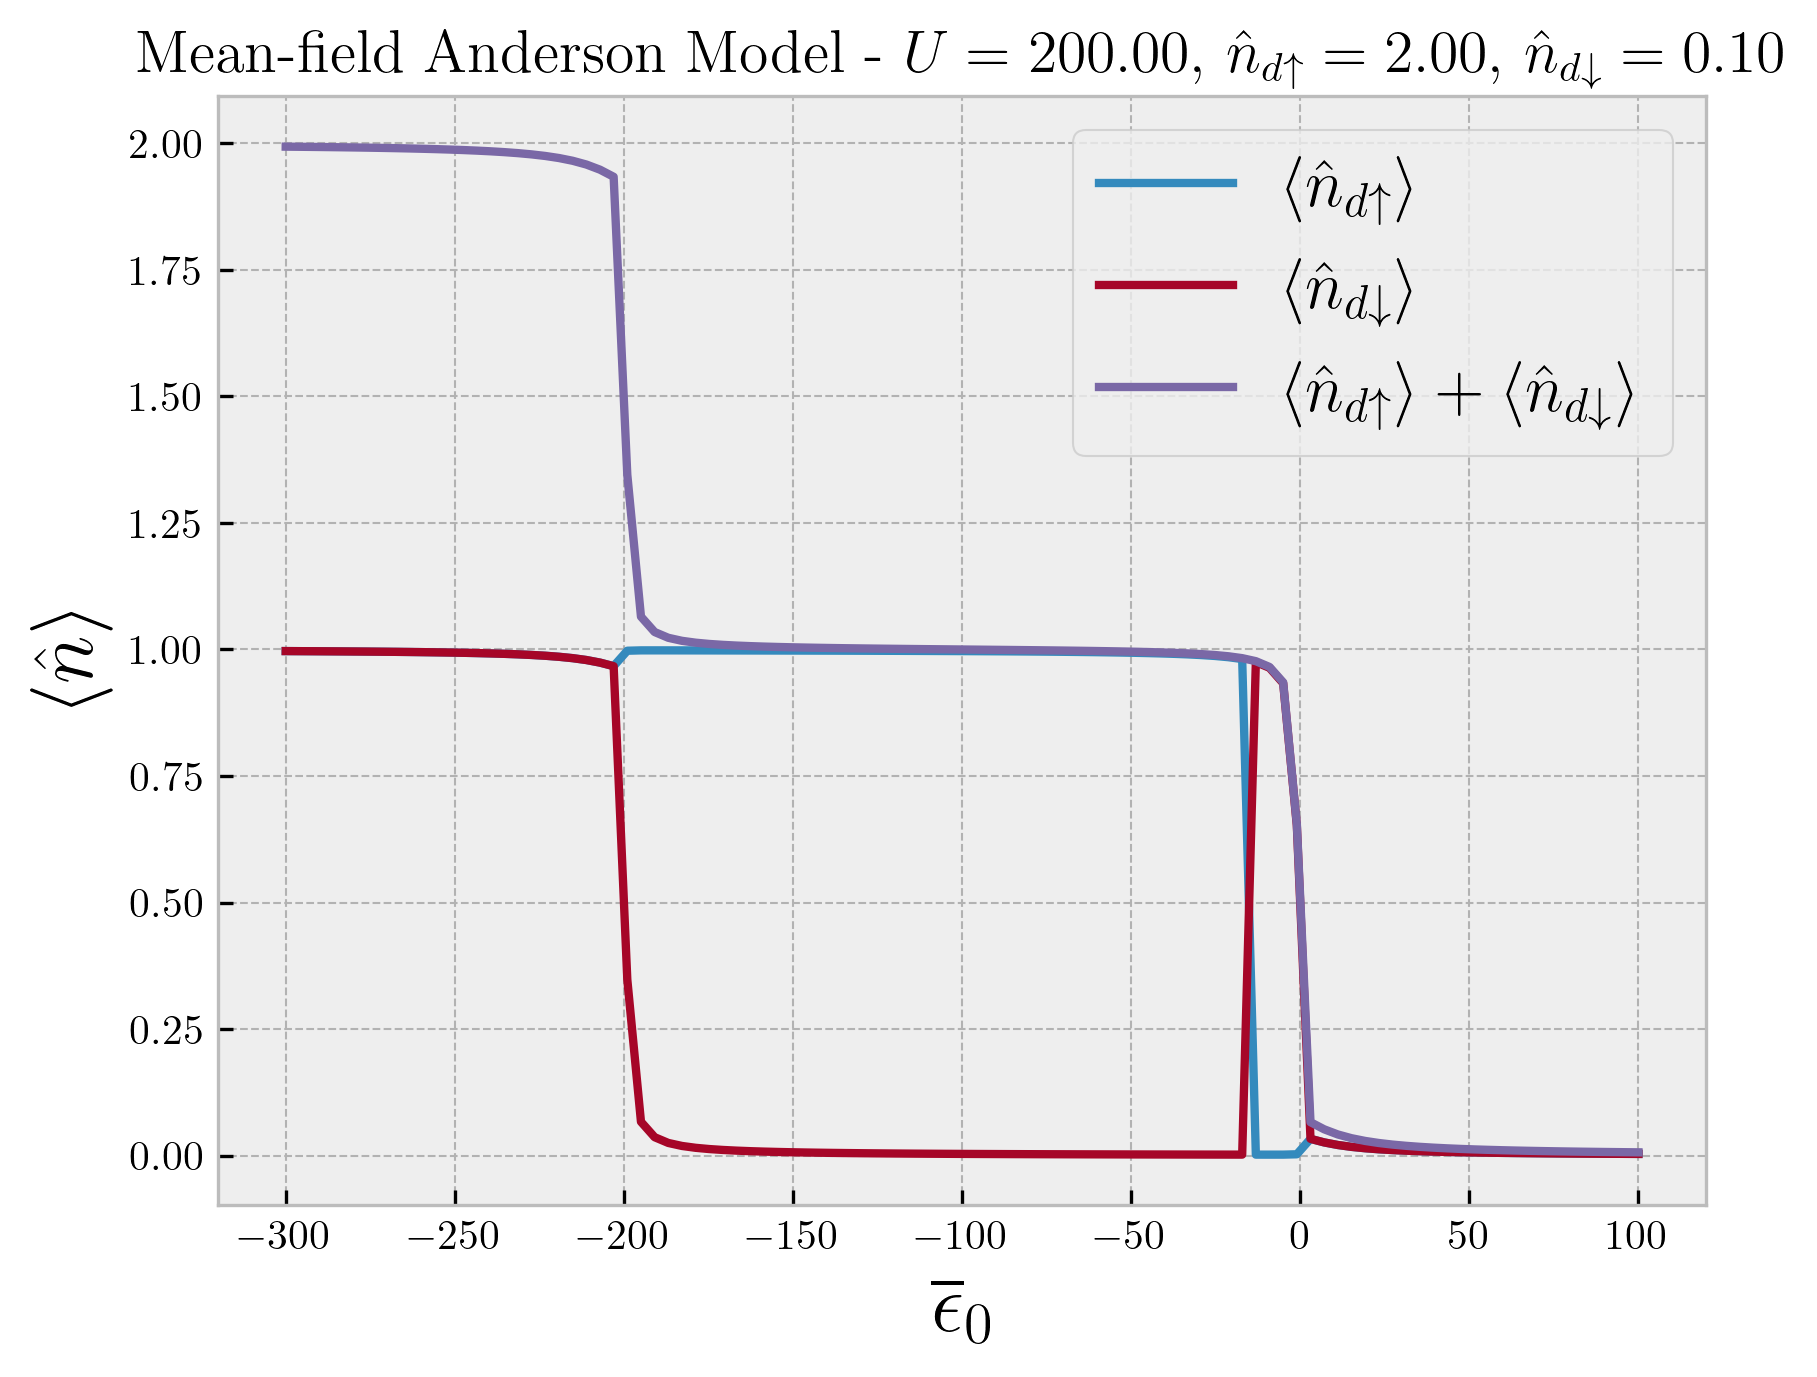
\includegraphics[width=\linewidth]{fig/plot-U_200-up_2.0-down_0.10.png}
\end{subfigure}
\end{figure}


\end{document}
